%% $RCSfile: proj_report_outline.tex,v $
%% $Revision: 1.2 $
%% $Date: 2010/04/23 02:40:16 $
%% $Author: kevin $

\documentclass[11pt
, a4paper
, twoside
, openright
]{report}

\usepackage{float} % lets you have non-floating floats

\usepackage{url} % for typesetting urls
\usepackage[numbers]{natbib}
\usepackage[toc,page]{appendix}
\usepackage{pdfpages}
\usepackage{color}
\usepackage{amsmath}
\usepackage{graphicx}
\usepackage{xcolor}
\usepackage{multirow}
\newcommand\todo[1]{\textcolor{red}{#1}}

\usepackage{listings}
\usepackage{color}

\definecolor{dkgreen}{rgb}{0,0.6,0}
\definecolor{gray}{rgb}{0.5,0.5,0.5}
\definecolor{mauve}{rgb}{0.58,0,0.82}

\lstset{frame=tb,
  language=Ruby,
  aboveskip=3mm,
  belowskip=3mm,
  showstringspaces=false,
  columns=flexible,
  basicstyle={\small\ttfamily},
  numbers=none,
  numberstyle=\tiny\color{gray},
  keywordstyle=\color{blue},
  commentstyle=\color{dkgreen},
  stringstyle=\color{mauve},
  breaklines=true,
  breakatwhitespace=true,
  tabsize=3
}

%
%  We don't want figures to float so we define
%
\newfloat{fig}{thp}{lof}[chapter]
\floatname{fig}{Figure}

%% These are standard LaTeX definitions for the document
%%                            
\title{Food Recommendations}
\author{Hai Quang Tran : 300224467}

%% This file can be used for creating a wide range of reports
%%  across various Schools
%%
%% Set up some things, mostly for the front page, for your specific document
%
% Current options are:
% [ecs|msor]              Which school you are in.
%
% [bschonscomp|mcompsci]  Which degree you are doing
%                          You can also specify any other degree by name
%                          (see below)
% [font|image]            Use a font or an image for the VUW logo
%                          The font option will only work on ECS systems
%
\usepackage[ecs,image]{vuwproject}

% You should specifiy your supervisor here with
\supervisors{John Clegg, Dr Xiaoying Gao, Dr Ian Welch}
% use \supervisors if there is more than one supervisor

% Unless you've used the bschonscomp or mcompsci
%  options above use
\otherdegree{Bachelor of Engineering with Honours}
% here to specify degree

% Comment this out if you want the date printed.
\date{}

\begin{document}

% Make the page numbering roman, until after the contents, etc.
\frontmatter

%%%%%%%%%%%%%%%%%%%%%%%%%%%%%%%%%%%%%%%%%%%%%%%%%%%%%%%

%%%%%%%%%%%%%%%%%%%%%%%%%%%%%%%%%%%%%%%%%%%%%%%%%%%%%%%

\begin{abstract}

This project explores recommendation techniques to integrate a recommender system into the web-centric mobile application What's On The Menu (WOTM). This recommendation system should be able to provide personalised recommendations to users based on the use case of ``Find Good Items" seen as items that a user will prefer based on their personal tastes towards food.

A user study has been conducted collecting a dataset containing 91 users, 100 food items, 4207 positive ratings, and 1638 negative ratings for an offline evaluation for recommender systems. A baseline predictor system recommending non-personalised items based on popularity was compared to four recommender systems, providing personalised recommendations. These systems were an Item-based SVD approach, a Single SVD approach, a Dual SVD approach, and a Hybrid CF approach. 

Overall, the Hybrid CF system was able to outperform every other system in terms of Accuracy, Precision, Area Under the Curve (ROC). In particular, the Hybrid CF approach was able to provide personalised recommendations at an accuracy of 87.06\%, outperforming the popularity baseline which provided non-personalised recommendations at an accuracy of 73.84\%, fulfilling the goal of ``Find Good Items".  

% The system will be tested using evaluation techniques (yet to be identified) on real user data. The user data will be collected during the course of Trimester 2, and will test the accuracy in addition to the performance and scalability of the system. This is yet to be determined. 
% The project looks at how a recommender system can be used to recommend food dishes to users based on personal food preferences, and previous binary rating patterns (Like/Dislike). 
\end{abstract}

%%%%%%%%%%%%%%%%%%%%%%%%%%%%%%%%%%%%%%%%%%%%%%%%%%%%%%%

\maketitle

% \chapter*{Acknowledgments}\label{C:ack} Any acknowledgments should go in here, between the title page and the table of contents.  The acknowledgments do not form a proper chapter, and so don't get a number or appear in the table of contents.

\tableofcontents

% we want a list of the figures we defined
\listoffigures

%%%%%%%%%%%%%%%%%%%%%%%%%%%%%%%%%%%%%%%%%%%%%%%%%%%%%%%

\mainmatter

%%%%%%%%%%%%%%%%%%%%%%%%%%%%%%%%%%%%%%%%%%%%%%%%%%%%%%%

% individual chapters included here
% 
\section{Literature Review}

FROM \cite{schafer2007collaborative}


The toolbox of recommender techniques has also grown beyond
collaborative filtering to include content-based approaches based on
information retrieval, bayesian inference, and case-based reasoning
methods
TODO: [132, 139].

These methods consider the actual content or attributes of the items to be recommended instead of or in addition to user rating patterns. 

Hybrid recommender systems [24] have also emerged as various recommender strategies have mature, combining multiple algorithms into composite systems that ideally build on the strengths of their component algorithms. Collaborative filtering, however,
has remained an effective approach, both alone and hybridized
with content-based approaches.

Research on recommender algorithms garnered significant attention in 2006 when Netflix launched the Netflix Prize to improve the state of movie recommendations. The objective of this competition was to build a recommender algorithm that could beat their internal CineMatch algorithm in offline tests by 10\%. It sparked a flurry of activity, both in academia and amongst hobbyists. The \$1 million prize demonstrates value that vendors place on accurate recommendations. 

\section{survey}
\cite{survey}
LOOK AT THIS MORE - REALLY GOOD

CONTAINS EVERYTHING. Can reference for problems of CF, different CF techniques etc.

+ As one of the most successful approaches to building recommender systems, collaborative filtering (CF) uses the known preferences of a group of users to make recommendations or predictions of the unknown preferences for other users.

+ main challenges, sparsity, scalability, synonymy, gray sheep, shilling attacks, privacy protection, etc.

+ Memory based, model-based, hybrid based

+ The fundamental assumption of CF is that if users  and  rate  items similarly, or have similar behaviors (e.g., buying, watching, listening), and hence will rate or act on other items similarly \cite{goldberg}

+ neighborhood/memory based deployed in amazon.com, and Barnes and Noble, because easy-to-implement, and highly effective. [6,7]

+ Limitations of memory-based CF,
 - similarity values based on common items, thus unreliable when data are sparse, and common items are therefore few. 
 
 To achieve better prediction performance and overcome shortcomings of memory-based CF algorithms, model-based CF approaches have been investigated.
 
 + Model-based CF techniques (Section 4) use the pure rating data to estimate or learn a model to make predictions [9]. Well-known model-based CF techniques include Bayesian belief nets (BNs) CF models [9–11], clustering CF models [12, 13], and latent semantic CF models [7].
 
 + Content based filtering make recommendations by analyzing content of textual information and finding regularities in the content. 

+ DIFFERENCE:  CF only uses the user-item ratings data to make predictions and recommendations, while content-based recommender systems rely on the features of users and items for predictions [15].

+ Hybrid CF techniques, such as the content-boosted CF algorithm [16] and Personality Diagnosis (PD) [17], combine CF and content-based techniques, hoping to avoid the limitations of either approach and thereby improve recommendation performance (Section 5).

+ User-based top- recommendation algorithms firstly identify the  most similar users (nearest neighbors) to the active user using the Pearson correlation or vector-space model [9, 27]

+ Item based were developed to address scalability problem of user based recommendations. 


\section{dimension}
\cite{dimension} 
\citeyear{dimension}
+ Collaborative filtering has been shown to produce high quality recommendations, but the performance degrades with the number of customers and products
+ New recommender system
technologies are needed that can quickly produce
high quality recommendations, even for very largescale
problems

+ Collaborative filtering is the most successful
recommender system technology to date, and is used
in many of the most successful recommender systems
on the Web, including those at Amazon.com and CDnow.com. 

+ neighborhood methods rely upon exact matches that cause algorithms to scarifice recommender system coverage. many customers have no correlation at all. Accordingly, preason NN may be unablet o make many product recommendations for a particular user. (reduced coverage) due to sparse ratings of neighbors. accuracy of recommendations may be poor because fairly little ratings data can be included. 

+ neighbourhood methods require computation that grows with number of customers and products. With millions of customers and prdoucts, typical system will suffer scalability problems. 

+ Synonym problem: different product names can refer to similar objects. Discovery of latent relationship from database may potentially solve synonym problem in recommender systems. 

+ Weakness of Pearson nearest neighbour for large sparse databases led us to explore alternative recommender systems. 


+ Attempts to address sparsity: incorporating semi-intelligent filtering agents into system. These agents evaluated and rated each product, using syntactic features. By providing a dense ratings set, they helped alleviate coverage and improved quality. However, did not address poor relationships among like minded but sparse-rating customers. 

+ Latent Semantic Indexing (LSI) to reduce dimensionality of customer-product ratings matrix. LSI is a dimensionality reduction technique that has been widely used in information retrieval (IR) to
solve the problems of synonymy and polysemy
(Deerwester et al. 1990).
By reducing the dimensionality
of the product space, we can increase density and
thereby find more ratings. 

+ LSI uses SVD as its underlying matrix factorization lagorihtm, maps incely into CF. 

+ The SVD-based approach was
consistently worse than traditional collaborative
filtering in se of an extremely sparse e-commerce
dataset.

+ However, the SVD-based approach
produced results that were better than a traditional
collaborative filtering algorithm some of the time in
the denser MovieLens data set

+ this technique leads to very fast online performance, requiring just a few simple arithmetic operations for recommendation. 
+ Computing SVD is expensive but can be done offline. 


\section{Itembased}
\cite{itembased}
\citeyear{itembased}|
Summary: 
Analyzes different item-based recommendation generation algorithms. Look into different techniques for computing item-item similarities (e.g. item-item correlation vs. cosine similarities between item vectors) and different techniques for obtaining recommendations from them (e.g. weighted sum vs regression model). Compare with basic k-nearest neighbour approach. Results suggest item-based algorithms provide dramatically better performance than user-based algorithms, while at the same time providing better quality than he best available user-based algorithms. 

+ user based producing high quality recommendations, performing many recommendations per second for millions of users and items and achieving high coverage in the face of data sparsity. In traditional CF, the amount of work increases with the number of participants in the system. 

+ New recommender system technologies are needed that can quickly produce high quality recommendations, even for very large-scale problems. To address these issues we explore item based CF. 

+ Bayesian networks are practical for environments which knowledge of user preferences changes slowly with respect to the time needed to build the model but are not suitable for environments in which user preference models must be updated rapidly or frequently.

+clustering techniques work by identifying groups f users who appear to have similar preferences. predictions for an individual can be made by averaging opinions of other users in that cluster. Clustering techniques usually produce less-personal recommendations than other methods, and often worse accuracy than nearest neighbour algorithms. [6] However, performance can be very good, since size of group that must be analyzed is much smaller. Can also be first step to shrink candidate set in a nearest neighbour algorithm. preclustering may be a worthwhile trade-off between accuracy and throughput. 
+Model approaches - don't have to compute similarity measures to form neighbourhoods so tend to produce faster recommendations. Looked at a model approach to pre-compute item-item similarities

+ Horting is graph-based technique which nodes are users, and edges between nodes indicate degree of similarity between two users [1]. 

+ Sparsity problem in Recommender system has been addressed in [23,11]  


\section{Tapestry}
\cite{goldberg1992using}
\citeyear{goldberg1992using}|

Summary: 
The novelty of Tapestry lies in its support for collaborative
filtering. Users are encouraged to annotate documents,
and these annotations can then be used for filtering. We
envision two types of readers for various classes of
documents. Eager readers will read all the documents in
the class in order to get immediate access. More casual
readers will wait for the eager readers to annotate, and
read documents based on their reviews. Experience with
NetNews suggests that there will not be a lack of readers
willing to be ’eager’ annotators.

\section{schafer}
\cite{schafer2007collaborative}
\citeyear{schafer2007collaborative}

The differing personalities exhibited by different recommender
algorithms show that recommendation is not a one-size-
fits-all problem. Specific tasks, information needs, and item domains
represent unique problems for recommenders, and design and evaluation
of recommenders needs to be done based on the user tasks to
be supported

This paper discusses a wide variety of the choices available and their implications to the important issues underlying recommenders and current best practices for addressing these issues. 

* Similarly,
nearly all rating data sets are strongly biased toward high ratings,
because users are careful to only choose to consume items
they suspect they will like.

+Item–item collaborative filtering, also called item-based collaborative
filtering, takes a major step in this direction and is one of
the most widely deployed collaborative filtering techniques today

+In a system that has more
users than items, it allows the neighborhood-finding to be amongst the
smaller of the two dimensions, but this is a small gain. It provides
major performance gains by lending itself well to pre-computing the
similarity matrix.

\section{scalable}
\cite{scalable}
\citeyear{scalable}

+ enhance neighborhood-based approach leading to substantial improvement of prediction accuracy, without meaningful increase in running time by removing global effects from data to make ratings more comparable, improving interpolation accuracy. Secondly, show how to simultaneously derive interpolation weights for all nearest neighbors, unlike previous approaches where each weight is computed separately. 

+ Efficient computation of an item-item neighborhoodbased
method requires precomputing certain values associated
with each item-item pair for rapid retrieval.

+ Common choices are the Pearson correlation coefficient and the closely related cosine similarity. Methods also differ by how they normalize or center data prior to activating interpolation rule (1) or (2).

+ Sarwar et al. [15] found that item-oriented approaches deliver better
quality estimates than user-oriented approaches while allowing
more efficient computations.

+ Neighborhood-based methods became very popular because
they are intuitive and relatively simple to implement.
In particular, they do not require tuning many parameters
or an extensive training stage. They also provide a concise
and intuitive justification for the computed predictions.

+ Standard neighborhood method concerns:
- similarity function directly defines interpolation weights is arbitary. Suppose that a particular item is predicted
perfectly by a subset of the neighbors. In that
case, we would want the predictive subset to receive
all the weight, but that is impossible for bounded similarity
scores like the Pearson correlation coefficient

+ Previous neighborhood methods do not account for interactions among neighbors. For example,
suppose that our items are movies, and the neighbors
set contains three movies that are highly correlated
with each other (e.g., sequelssuch as “Lord of the
Rings 1–3”). An algorithm that ignores the similarity
of the three movies when determining their interpolation
weights, may end up essentially triple counting the
information provided by the group.

+ By definition, the interpolation weights sum to one, which may cause overfitting. '

+ In recent work [2], we overcame most of these shortcomings,
but the resulting algorithm was several orders
of magnitude slower than previous neighborhood-methods,
thereby limiting its practical applicability.

\section{Toward}
\cite{toward}
\citeyear{toward}

+ overview of content-based, collaborative, and hybrid recommendation approaches and limitations. 

+ Content-based recommendations: user will be recommended items similar to the ones the user preferred in the past. Tries to understand the commonalities among the movies that the user has rated highly in the past (specific actors, directors, genres, subject matter etc). Then, only the movies that have a high degree of similarity to whatever the user's preferences are would be recommended. 

+ Problems with content-based recommendations.
    - Limited by features that are explicitly associated with objects. Hard to extract features or have to manually put them in.
    - Cannot tell difference between good and bad items because contain same feature set
    - Overspecialization : limited to being recommended items that are similar to those already rated. 
    - User should be presented with a "range of options" (Diversity is important in recommender systems) 
    - Need to rate sufficient number of items before it can understand your preferences. 

+ collaborative recommendations: user will be recommended items that people with similar tastes and preferences liked in the past; Unlike content-based recommendation methods, collaborative recommender systems (or collaborative filtering systems) try to predict the utility of items for a particular user based on the items previously rated by other users.

+ hybrid approaches: methods combine collaborative and content-based methods. 

+ rating-based recommenders since it constitutes the most popular approach to recommender system


+ Grundy system would build individual user models
and use them to recommend relevant books to each user.
Later on, the Tapestry system relied on each user to
identify like-minded users manually [38]. GroupLens [53],
[86], Video Recommender [45], and Ringo [97] were the
first systems to use collaborative filtering algorithms to
automate prediction

+One problem with using the weighted
sum, as in (10b), is that it does not take into account the fact
that different users may use the rating scale differently. The
adjusted weighted sum, shown in (10c), has been widely
used to address this limitation. In this approach, instead of
using the absolute values of ratings, the weighted sum uses
their deviations from the average rating of the corresponding
user.

+ Memory based is using heuristics to find similarity between items or users

+ Model based is using probabilistic approach where unknown ratings will be predicted to users based on their previous rating patterns. cluster models and Bayesian networks. 
Clustered models cluster like-minded users into classes. The number of classes and parameters of the model are learned from the data.
Bayesian network represents each item in domain as a node in the network. Each state of the node correspond to possible rating values for each item. Both structure of network and the conditional probabilities are learned from the data. Limitations of this approach is that each user can be custered into a single cluster, whereas some recommendation applications may benefit from the ability to cluster users into several categories at once. For example,
in a book recommendation application, a user may be
interested in one topic (e.g., programming) for work
purposes and a completely different topic (e.g., fishing)
for leisure.based on a model
learned from the underlying

+ model-based methods outperform memory-based
approaches in terms of accuracy of recommendations.


+There have been several other model-based collaborative
recommendation approaches proposed in the literature. A
statistical model for collaborative filtering was proposed in
[105], and several different algorithms for estimating the
model parameters were compared, including K-means
clustering and Gibbs sampling. Other collaborative filtering
methods include a Bayesian model [20], a probabilistic
relational model [37], a linear regression [91], and a
maximum entropy model [75]. More recently, a significant
amount of research has been done in trying to model the
recommendation process using more complex probabilistic
models. For instance, Shani et al. [96] view the recommendation
process as a sequential decision problem and
propose using Markov decision processes (a well-known
stochastic technique for modeling sequential decisions) for
generating recommendations. Other probabilistic modeling
techniques for recommender systems include probabilistic
latent semantic analysis [47], [48] and a combination of
multinomial mixture and aspect models using generative
semantics of Latent Dirichlet Allocation [64]. Similarly, Si
and Jin [99] also use probabilistic latent semantic analysis to
propose a flexible mixture model that allows modeling the
classes of users and items explicitly with two sets of latent
variables


+Furthermore, Kumar et al. [55] use a simple
probabilistic model to demonstrate that collaborative filtering
is valuable with relatively little data on each user, and
that, in certain restricted settings, simple collaborative
filtering algorithms are almost as effective as the best
possible algorithms in terms of utility.

+The pure collaborative recommender systems do not
have some of the shortcomings that content-based systems
have. In particular, since collaborative systems use other
users’ recommendations (ratings), they can deal with any
kind of content and recommend any items, even the ones
that are dissimilar to those seen in the past

+COLLABORATIVE FILTERING PROBLEMS

 + New User Problem
    must learn user's preferences from ratings that the user gives. 
    Several approaches have been proposed to address this pobrlem, most being hybrid approaches. These techniques use strategies that     are based on item popularity, item entropy, user personalization, and
    combinations of the above [83], [109].
    
 + New Item Problem
until the new item is
rated by a substantial number of users, the recommender
system would not be able to recommend it

+ Sparsity

In any recommender system, the number of ratings already
obtained is usually very small compared to the number of
ratings that need to be predicted. Effective prediction of
ratings from a small number of examples is important. Also,
the success of the collaborative recommender system
depends on the availability of a critical mass of users. 

+ TO OVERCOME SPARSITY
- use user profile information when calculating user similarity. That is, two users could be considered similar not only if
they rated the same movies similarly, but also if they belong to the same demographic segment. For example, [76] uses the gender, age, area code, education, and employment
information of users in the restaurant recommendation
application
- A different
approach for dealing with sparse rating matrices was used
in [11], [90], where a dimensionality reduction technique,
Singular Value Decomposition (SVD), was used to reduce
the dimensionality of sparse ratings matrices


+ HYBRID APPROACHES
which
helps to avoid certain limitations of content-based and
collaborative systems [8], [9], [21], [76], [94], [100], [105].

1. implementing collaborative and content-based
methods separately and combining their predictions,
2. incorporating some content-based characteristics
into a collaborative approach,
3. incorporating some collaborative characteristics into
a content-based approach, and
4. constructing a general unifying model that incorporates
both content-based and collaborative
characteristics.
\chapter{Introduction}\label{C:intro}

\todo{Feedback to do from Ian}
\begin{enumerate}
 \item \todo{People get bored + want new foods to try that they might like}
 \item \todo{WOTM idea -> Contraints is binary decisions}
 \item \todo{Can we use off the shelf recommender system?}
\end{enumerate}

With the numerous food options around us, it is often difficult to decide what to eat. On some days we may feel like eating our favourite foods, but on other days we could feel more explorative, wanting to try something new. There are many factors that determine our decisions on what we want to eat such as our preferences, our current mood, and what food providers are nearby. Other factors that may contribute is the price of the food dish, the cuisine type, the meat type, and so forth. Additionally, a subset of users have food intolerances which restrict their food options, further making the food decision process difficult.

\todo{There is a jump here, where di recommender system come from?}
\todo{Talk about the Long Tail problem?}
% The Long Tail problem in the context of recommender
% systems has been addressed previously in [3] and [4]. In
% particular, [3] analyzed the impact of recommender systems on
% sales concentration and developed an analytical model of
% consumer purchases that follow product recommendations
% provided by a recommender system. The recommender system
% follows a popularity rule, recommending the bestselling products
% to all consumers, and they show that the process tends to increase
% the concentration of sales. As a result, the treatment is somewhat
% akin to providing product popularity information. The model in
% [3] does not account for consumer preferences and their
% incentives to follow recommendations or not. Also [3] studied the
% effects of recommender systems on sales concentration and did
% not address the problem of improving recommendations for the
% items in the Long Tail, which constitutes the focus of this paper.
% In [4], a related question has been studied: to which extent
% recommender systems account for an increase in the Long Tail of
% the sales distribution. [4] shows that recommender systems
% increase firm’s profits and affect sales concentration. 

\todo{Check this again (Massive massive brain dump)}
It can be difficult to find good food dishes to eat. There are several factors that can influence our decisions. These factors must be considered in a recommender system that is able to provide personalised recommendations to each user. Taste is subjective, people are different. \todo{ introduce earlier} The main goal of this project is to present a base recommender system that is able to ``Find Good Items" for each user, providing personalised recommendations that can be integrated for the application What's On The Menu (WOTM). The challenge in this project, lays within the factors that determine a ``Good Item" for a user, and providing a recommender system that meets the needs of the users. The first is to find an algorithm that will be able to achieve this goal. There are a vast range of techniques that are used for recommendations, however, each algorithm fits a specific context, and relies on conditions that are needed. There are always trade-offs that need to be considered. Factors that should be considered are the scalability, the accuracy, the cold start problem, the sparsity, and the computation complexity while considering the user experience (keeping in mind that users must be able to achieve their goal of finding good items.) So what defines a good item? Is it the novelty? the contents of the food dishes? how others feel about the dish? the price and so on? In addition to this, a main problem is not having enough data from users. How can we provide recommendations to the users when they do not indicate enough information to provide personalised recommendations? Another issue is being able to develop a recommender system that can integrate with the existing WOTM application. \todo{In addition, there lacks research in the recommender field of systems that look at only using Binary data driven by usability, in this case, like and dislikes. Most research looks at a more fine grained rating system such as from 1-10 stars. Using only binary data for ratings is a problem in itself. Despite this, the recommender system evaluation process is a problem in itself. How do we know that the recommender system meets our needs? Binary driven by usability -> Like and Dislike}

\section{Motivation}

\todo{There is limited research on binary recommender systems}

\todo{Add motivation}
\subsection{Algorithm is dependent on each use case}
\subsubsection{Data that can be collected}
\subsection{Find Good Items}
\subsection{Novelty/Serendipity}
\subsection{Commercial Product that can be iterated in the future.}
\section{Project Objectives}

\todo{Add project goals}


\todo{Is this the reason question or overall project goal?}
\todo{good reasons \cite{memorybased} \citeauthor{memorybased}} 
 Every year several new techniques are proposed and yet it is not clear which of the techniques work best and under what conditions. 
The prediction accuracy of the different algorithms depends on the number of users, the number of items, and density, where the nature and degree of dependence differs from algorithm to algorithm.There exists a complex relationship between prediction accuracy, its variance, computation
time, and memory consumption that is crucial for choosing the most appropriate recommendation algorithm.


What’s On The Menu (WOTM) is a web-centric mobile application that is focused on recommending food dishes to users based on their personal food preferences (e.g. Meat preference, Cuisine Preference, Food Preference etc), previous actions such as likes/dislikes, and other factors such as location, price, and so forth. These personalised recommendations are important as it saves time for users and allows users to explore preferred food options they otherwise might not have discovered alone. 

\section{\todo{What's On The Menu Overview}} \label{section:wotm}

What's On The Menu (WOTM) is a system that aims at providing personalised food recommendations to users. It is currently in development and was created by John Clegg from Summer Of Tech. WOTM consists of two components: WOTM Web and WOTM API. WOTM Web is the front-end of the application that deals with interactions in the client browser. WOTM API is the back-end of the application that deals with the application logic and management of data. \todo{ I will be extending the existing system by creating an additional component called WOTM Recommendations. This component will connect to the other components to provide recommendations to the users, and will manage anything related to the recommendation system. }

Existing applications such as Yelp \cite{yelp} and Foursquare \cite{foursquare} have similar concepts but lack personalised recommendations for food dishes. These applications focus on a broader scope such as popular restaurants, coffee places, activities, and so forth. This can often lead to a cluttered interface, affecting the user experience, and may provoke confusion in users. Food spotting is an application that focuses on food dishes but does not provide personalised recommendations to users. Instead, they show popular food dishes and focus on crowd-sourcing, relying on users to upload food dishes. What's On The Menu (WOTM) differs as the goal is to recommend personalised food recommendations to the low level granularity of a food dish. Specifically, the personalised recommendations will be provided through a recommender system aimed towards the use case of finding ``Good Items" based on the user. This report, specifically focuses on a type of recommender algorithm called Collaborative filtering. 

Collaborative filtering is a popular recommendation technique used to recommend items to users based on previous rating patterns and the behaviours of others \cite{itembased, schafer2007collaborative, survey}. 

\todo{State explicit goals}
The aim of this project is to provide a base recommendation engine that will be able to provide recommendations for the web-centric mobile application ``What's On The Menu" (WOTM). In particular, the project mainly focuses on Collaborative filtering algorithms, suitable for the application to be used in a commercial environment. The main focus of the project is on the recommendation engine. This involves the algorithms that will be used, the data that will be collected, and how the existing WOTM application will communicate with the recommendation engine. 
For clarification, we explicitly state the goals of the project in the following points:
\todo{redo all of this}
\begin{itemize}
	\item{Consider a recommendation system that is able to provide accurate recommendations to users for the use case of ``Find Good Items"}
	\item{Given binary explicit rating data, provide accurate recommendations}
	\item{Develop a Food Recommender System}
	\item{Integrate into WOTM}
	\item{Develop/Implement algorithm}
	\item{Create data set}
	\item{Evaluate them}
\end{itemize}

% The goal of this project is to find which types of collaborative filtering algorithms best suit the WOTM application. Suitability of these algorithms will be considered on factors that are important for WOTM. The recommender system will have to account for a range of factors from the user experience, the accuracy of the recommendation system, and the speed/performance that the system can provide recommendations to users. This project aims to explore this, by implementing different types of collaborative filtering techniques to recommend food to users based on their personal preferences and previous behaviours.


\chapter{Background \& Related Work}\label{C:background}

\section{Collaborative Filtering}

Collaborative filtering (CF) is a popular technique that has been successfully used in recommender systems \cite{itembased, schafer2007collaborative, survey}. The main idea behind collaborative filtering is that rating behaviours of others can be used to predict items that the active user will be interested in. Intuitively, this algorithm stems from the assumption that users having similar opinions for items that they have both rated tend to have similar tastes to each other, having similar opinions about other items  \cite{schafer2007collaborative}. For example, most of us have friends with similar opinions and tastes to us. Perhaps you and a friend both like eating chicken sandwiches. Since you and your friend have similar tastes, your friend may then be able to suggest to you another food dish that you might enjoy such as duck with rice. Collaborative filtering uses the same concept, but usually on a larger scale. 

\begin{figure}
\centering
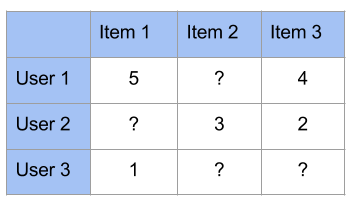
\includegraphics[scale=0.7]{images/User-Item}
\caption{A user-item ratings matrix containing scaled ratings from 1-5.}
\label{fig:matrix}
\end{figure}

Users express their preferences for a variety of items through ``ratings" which can be in different forms such as 1-5 star ratings, or binary scale ratings such as likes/dislikes. These ratings are typically represented as a (User, Item, Rating) triplet. These ratings can be represented in the form of a matrix, where the rows of the matrix are users, the columns of the matrix are items, and the ratings are represented inside the matrix (See Figure \ref{fig:matrix}). Since the matrix contains sets of rating triplets, the (User, Item) pairs will exist where a user has not yet rated the item, thus the matrix is usually sparse.

Since the matrix can be sparse, collaborative filtering can struggle when there are not enough ratings to provide accurate recommendations to users. Sparse ratings can also lead to another issue called the ``Cold Start' problem, where ratings for new items or new users have not yet been collected. 

% THIS CAN BE A SECTION IN DESIGN DECISIONS?
\todo{Add Content based filtering description}
% \textcolor{red}{TODO: Take this out or leave in?}

% In this context, content-based filtering is superior \cite{koren2009matrix}.

% The advantage of collaborative filtering is that it does not require domain knowledge of items or users to provide recommendations. It purely focuses on the previous behaviours of users and their rating history, providing recommendations that are generally more accurate than content based filtering \cite{koren2009matrix, schafer2007collaborative}. 

% Collaborative filtering is preferred over content based filtering, a technique where items are recommended based on learning users preferences from previous rating patterns of the user, and recommending similar items based on the attributes of those items. Additionally, content based filtering is prone to recommending only a small subset of items, since it recommends items based on attributes of the items, leading to overspecialization thus restricting variety \cite{toward}. Another problem of content-based filtering is that it is difficult to extract features from the items and users, and manually labelling these features may not be practical \cite{toward}. Traditional collaborative filtering are able to address these concerns since attributes are ignored, and recommendations are based on actions of other users, providing a range of recommendations that are not restricted to specific attributes \cite{koren2009matrix}. For these reasons, we chose to not address content-based filtering, but explain it because hybrid collaborative filtering approaches use it. 

Using the matrix, a list of top N recommendations is usually given to the user representing the items they will like, computed through collaborative filtering techniques. For example, the active user may be recommended 10 food dishes that might be of interest to them whenever they log into WOTM.  

% \textcolor{red}{TODO: Take this out or leave in?}

% Collaborative filtering is preferred over content based filtering, a technique where items are recommended based on learning users preferences from previous rating patterns, recommending items based on the attributes and the preferences learnt from the user profile. Additionally, content based filtering is prone to recommending only a small subset of items, since it recommends items based on attributes of the items, leading to overspecialization thus restricting variety \cite{toward}. Another problem of content-based filtering is that it is difficult to extract features from items and users, and manually labelling these features may not be practical \cite{toward}. 


% The advantage of collaborative filtering is that it does not require domain knowledge of items or users to provide recommendations. It purely focuses on the previous behaviours of users and their rating history, providing recommendations that are generally more accurate than content based filtering \cite{koren2009matrix, schafer2007collaborative}. 

% Traditional collaborative filtering are able to address these concerns since attributes are ignored, and recommendations are based on actions of other users, providing a range of recommendations that are not restricted to specific attributes \cite{koren2009matrix}. However, in the 'cold start' problem, content-based filtering is superior than collaborative filtering because it does not rely on the opinion of other users \cite{koren2009matrix}.

% For these reasons, we chose to not address content-based filtering, but explain it because hybrid collaborative filtering approaches use it. 

There are three main areas of CF, these areas are memory-based CF techniques, model-based CF techniques, and hybrid-based CF techniques. In this project, we will be examining in particular, the neighbourhood methods which are a form of memory-based CF techniques, and latent factor models which are a form of model-based CF techniques \cite{survey, koren2009matrix}. Neighbourhood methods, and Latent factor models will be explained in the following sections. 

% \section{Challenges}
% \subsection{Cold Start}
% \subsection{Data Sparsity}
% \subsection{Synonyms}
% \subsection{Scalability}
% \subsection{Grey Sheep}
% \subsection{Shilling attacks}
% \subsection{Diversity and the Long Tail}

\section{Neighbourhood Methods}

Neighbourhood CF methods can be classified into the class of memory-based CF techniques because they use the entire or a sample of the ratings matrix to find the similarity between users (or items) through a heuristic \cite{memorybased, schafer2007collaborative}. The main idea of this approach is to use the ratings matrix to compute the similarity between users (or items) which are then used for recommendations. This typically involves finding all user-user similarities (or item-item similarities) and using neighbourhood algorithms such as K-Nearest Neighbour to find the K most similar users (or items), referred to as neighbours. The K most similar users (or K most similar items) are then used to predict how the active user will feel about specific items, thus being able to make recommendations for the active user based on their neighbours. Since these neighbours may contain quirky characteristics that are not common among the users, methods tend to take the weighted average of the neighbours ratings or simple weighted average to generate predictions for the active user \cite{survey}. 

Common similarity measures that are used are Pearson's Correlation, Cosine similarity, Euclidean distance, Jaccardian similarity and so forth, finding similar users to the active user (or similar items that the active user has previously performed actions on). The most common neighbourhood method that is used to find the most similar users (or items) is the K-Nearest Neighbour algorithm. This algorithm finds the K-nearest neighbours based on a heuristic, in this case, the similarity measure. Other neighbourhood algorithms are K-Means, K-d Trees, and Locality Sensitive Hashing \cite{survey}. 

% A key problem of collaborative filtering is how to combine and weight the preferences of user neighbors. Sometimes, users can immediately rate the recommended items. As a result, the system gains an increasingly accurate representation of user preferences over time.

The following section explains the difference between user-based CF and item-based CF.

% +Advantages
%     -   explain
%     - easy to create etc
%     - easy facilitation of new data
%     - content independence of itemsbeing reocmmended
%     - good scaling with co-rated items
% +Disadvantages
%     - performance decrease with sparse data
%     - scalability and problems with large datasets
%     - adding new items required inclusion of the new item and re-insertion of all elements in the structure



\subsection{User-based Collaborative Filtering}

\todo{Fix this, too repetitive}
User-based CF uses a similarity measure to find like-minded individuals that are similar to each other, producing recommendations to the active user based on ratings of similar users. The defining characteristic of user-based CF is based upon similarities between users \cite{mahoutaction}. A concrete example would be two users that rated the same food dishes similarly, the first user has indicated that they like the Big Mac and the Whopper Burger; similarly, the second user indicated that they like the Big Mac too, therefore, since these two users previous ratings are similar (both like Big Macs), they are to be considered similar; we can then recommend to the second user that they should try the Whopper Burger, since the users have similar opinions about the item. User-based CF has the same idea with the example, but typically works better on a larger scale - more ratings, more users, and more items are involved. 


\subsection{Item-based Collaborative Filtering}

Another approach that is commonly used is item-based CF. Instead of finding users that are similar to each other, item-based CF focuses on recommending items that are similar \cite{mahoutaction}. Similar items are extracted by the rating patterns of other users rather than the attributes of the item - two items are considered similar if users rate them similarly \cite{schafer2007collaborative}. For example, a user could have previously liked the following dishes: a chicken sandwich, chicken nuggets, and chicken soup. Item-based CF will find similar items that the user has previously rated by using a similarity measure. By using this technique, it may recommend items based on the users previous interests, suggesting new items such as chicken salad, or a chicken burger since users who like the previous dishes of the active user tend to like these dishes. This is the main idea behind item based collaborative filtering. 


\section{Latent Factor Methods}


% \textcolor{red}{
% Latent factor models, such as matrix factorization (aka, SVD), comprise
% an alternative approach by transforming both items and users to the same latent factor
% space. The latent space tries to explain ratings by characterizing both products
% and users on factors automatically inferred from user feedback \cite{koren2011}
% }

Latent factor models can be classified into the class of model-based CF techniques because they try and explain ratings by automatically inferring meaningful information from users previous rating patterns which are then used to make intelligent predictions based on this meaningful information \cite{survey}. For example, these methods automatically try and learn about the properties or characteristics of the items such as the food dishes, and learn how much the user likes each of these properties, also known as latent factors \cite{koren2011}. 

Matrix factorization is seen as one of the successful techniques of latent factor models \cite{memorybased, koren2009matrix}. Singular Value Decomposition is a matrix factorization technique that is well-known and can be applied to the CF domain, identifying latent semantic factors \cite{koren2009matrix}. The following section talks about the matrix factorization technique of Singular Value Decomposition and how it is used to recommend items to users. 

%  These methods have become popular in
% recent years by combining good scalability with predictive
% accuracy. In addition, they offer much flexibility for modeling
% various real-life situations

\subsection{Matrix Factorization}

\todo{Fix this section - explain that it only maps to rated items}

In the context of this project, the main goal of Singular Value Decomposition (SVD) is to train a model to learn what properties of a dish that a user likes. This can be used to predict how a user may feel about another dish by looking at the properties that are inferred from that dish.
\todo{Clarification about the context of SVD - From Simon Funk and not mathematical one.}


SVD decomposes the ratings matrix, where both users and items are mapped to a joint latent factor space of dimensionality \begin{math} f \end{math} - the space containing the inferred properties of the food dishes, and how the users feel about those properties. The latent space tries to explain the ratings given from the ratings matrix by considering these inferred latent factors. These latent factors are represented in the form of an item vector \begin{math} q_{i} \in \mathbb{R}^f  \end{math} and a user vector \begin{math} p_{u} \in \mathbb{R}^f  \end{math} where \begin{math} i \end{math} is a given item and \begin{math} u \end{math} is a given user. The vectors contain a specified number of factors for each item and user, which are used to predict how the user may feel about other items that they have not yet rated \cite{koren2009matrix}. Factors in the item vectors could be dimensions regarding the properties of the items. An example for food dishes are item vectors that discover factors measuring obvious dimensions in the food dish such as the ingredients, spice levels, cuisine type, or meat type; less defined dimensions such as carbohydrates, or uninterpreted dimensions in the food dish \cite{koren2009matrix}. User vectors contain factors that measure the extent that the user likes those factors which are the properties that are inferred from the food dishes \cite{koren2009matrix}. These factors in \begin{math} q_{i} \end{math} and \begin{math} p_{u} \end{math} can be positive or negative, representing how much the properties contained within each dish, and how much the user likes those properties. 

These feature vectors contain a specified number of factors for each item and user, which are used to predict how the user may feel about other items that they have not yet rated \cite{koren2009matrix}. For this model, a user's predicted rating for a dish would be the dot product of the food dish vector, and the user vector \begin{math} q_{i}^T p_{u} \end{math}. This approximates to the active user's rating of the current item, denoted by \begin{math} r_{ui} \end{math}, leading to the estimate \cite{koren2009matrix}

\begin{equation}\label{eq:1}\tag{1} \widehat{r} = q_{i}^T p_{u} \end{equation}.

% \begin{equation}\label{}

Since the user vector represents how much they like about the characteristics of the dish, and the item vector represents the portion of how much of the dish contains those properties \cite{koren2009matrix}, we can use the dot product - multiplying the dish containing a specific property from the item vector with how much the user likes that property from the user vector, and repeat this for all elements in the vectors to see the overall interest that the user has of the dish. This represents the active user's interest about the overall dish and is used to estimate the rating a user will give to the item. 

Now that we understand how the predicted ratings for an item and user are computed, you may be wondering how we infer the item and user vectors explained above. 

To do this, the system learns the model by fitting the previously observed ratings. However, directly modelling the observed ratings can lead to over fitting, being overspecialized leading to inaccurate future predictions.

To prevent this, the idea is to use a regularized model that is used to generalize the previous ratings in a way that is able to predict future unknown ratings. To learn the vectors for the items and users, the system uses an equation that minimizes the regularized squared error on the set of known ratings.

\begin{equation}\label{eq:2}\tag{2}
\displaystyle min_{q*,p*} \sum_{ (u,i) \in K} (r_{ui} - q_{i}^T p_{u}) + \lambda (\| q_{i} \|^2 + \| p_{u} \|^2 )
\end{equation}

\begin{math} K \end{math} represents the training set from the rating matrix where \begin{math} r_{ui} \end{math} is known for the user, item pairs \begin{math} (u,i) \end{math}. The constant \begin{math}\lambda\end{math} controls the regularization used to penalize the magnitudes to avoid over fitting, and is typically tuned by cross-validation. Minimization is performed by Alternating Least Squares \cite{koren2011}  which is detailed below. 

% In order to fill in these missing values, singular value decomposition is used to learn feature vectors (factors) of items and users. The items feature vectors represent the characteristics of the items, in this case: dishes. User feature vectors represent how much the user prefers these characteristics of the dish. However, since the user item matrix contains many missing values it is unwise to train directly from it, as it is highly to cause overfitting. You can use inductions? to fill in these will values, but it takes up space, and may cause a lot of error if you get it wrong. Therefore you use the ratings given, but use lambda to determine the strength of those ratings. From there you can learn these algorithms. 

% Now you may be wondering how these feature vectors are learnt. These feature vectors are learnt through an equation, in which we minimise the square error to find the best latent features. By doing this, we use two algorithms to find the minimum error and to find the appropriate feature vectors.

\subsubsection{Alternating Least Squares}

The main purpose of Alternating Least Squares (ALS) is to find the minimum error from equation \ref{eq:2}, which is used to learn the factors in each of the vectors based on the rating matrix. ALS works to find the item and user vectors by initializing the vectors with random values depending on how many factors are specified. From this, it fixes values of one of the vectors first such as the item vector, then computes and reassigns values of the user vector according to the minimization equation, shown as equation \ref{eq:2} above. After this, it alternates - the user vector values are now fixed, and the re-computation of the item feature values occur, trying achieve the result of the smallest value for the minimization equation. This technique keeps alternating between fixing the vector values, until there is a convergence where the values in the two vectors no longer change the minimization equation, or there is small changes, hence the name Alternating Least Squares. This is used to find the minimum error from the equation mentioned above and to learn the factors in each of the vectors. 

\section{Related Work}

The term ``collaborative filtering' was first introduced in \citeyear{goldberg1992using} by \citeauthor{goldberg1992using} to describe the technique used in Tapestry, one of the earliest known recommender systems \cite{koren2009matrix,  goldberg1992using, itembased, survey}.

Tapestry \cite{goldberg1992using} was created to handle electronic documents and used manual collaborative filtering, allowing users to query information based on other's opinions about the documents. These opinions were in the form of annotations or replies which users were encouraged to make on documents to increase probability of relevant results returned from queries \cite{schafer2007collaborative}. Tapestry relied on opinions from a small community such as an office workgroup, where each person's opinion was trusted. Larger communities could not rely on every person knowing each other, leading to new collaborative filtering techniques being developed \cite{itembased}. 

More recommender systems emerged as value was seen in the potential to increase sales from recommendations - customers may purchase suggested items that they might not have seen otherwise \cite{schafer2007collaborative}. Perhaps the most popular recommender system in the late 1990's was used in Amazon.com, collecting user purchase history, browsing history, and recently viewed items to recommend items that the user may buy \cite{schafer2007collaborative}. Other recommender systems consisted of Jester \cite{goldberg} for jokes, and Ringo \cite{ringo} for music.
% /cite{schafer2007collaborative, toward}
GroupLens \cite{grouplens} were the first to introduce a neighbourhood collaborative filtering technique. Building upon the Tapestry concept, GroupLens created an automated user based collaborative filtering technique for recommending Usenet articles that users may be interested in. The advantage of neighbourhood methods is that they are intuitive, easy to implement, and produce highly effective results \cite{survey, scalable}. Despite providing accurate recommendations, user-based collaborative filtering techniques were computed in real time and their performance would degrade as more users and items were added to the system, leading to scalability and performance issues \cite{dimension, itembased, evaluationitem}.

This required collaborative filtering techniques that could easily scale and still produce high quality recommendations, leading to the exploration of item-based collaborative filtering. Item-based collaborative filtering techniques were developed to address scalability limitations of the user-based techniques \cite{survey}. \citeauthor{itembased} analyzed various item-based recommendation algorithms, computing item-item similarities and comparing the accuracy with traditional KNN user based collaborative filtering techniques \cite{itembased}. \citeauthor{itembased} found that items remained fairly static in the system, whereas user behaviours and preferences would often change. Because items were found mostly static, it meant precomputation could occur for item similarities. By having precomputed item similarities, traditional item-based collaborative filtering can then be applied, thus performance and scalability would be increased \cite{scalable}.

Other techniques such as model based collaborative filtering have also been investigated to overcome the performance and scalability issues. Well known model based techniques include Bayesian belief nets \cite{baysian}, clustering models \cite{clustering}, and latent semantic models \cite{latent}. These models are based on learning patterns from users previous actions to predict new items, and are expensive but can be built offline allowing high scalability. The resulting model is "very small, very fast, and essentially as accurate as nearest neighbor methods" \cite{itembased}. \citeauthor{itembased} found Bayesian networks to be practical in the context where user ``preferences change slowly with respect to the model" \cite{itembased}. However, these models are not suitable for environments where the user preference model should be updated rapidly or frequently. Since model based approaches do not have to compute similarity measures to form neighbourhoods, they tend to produce faster recommendations and outperform neighbourhood models in terms of accuracy of recommendations \cite{toward, itembased}. 

Although collaborative filtering is considered to be one of the most successful approaches to recommender systems \cite{survey, toward}, they suffer from the problem of data sparsity \cite{toward, survey, itembased, koren2009matrix, koren2011, dimension}. Data sparsity is when only a small subset of user ratings on items are recorded, leading to an insufficient number of ratings to produce accurate recommendations. Data sparsity specifically tends to appear in the ``cold start' problem, where new items or new users are entered into the system, but not enough information is supplied to produce accurate recommendations since recommendations are based on common items or users \cite{survey}.

To alleviate this problem, hybrid approaches were investigated that combined collaborative filtering and other recommender techniques such as content based filtering. \citeauthor{toward} suggested creating user profiles such that demographic information could be included in similarity measures to provide extra content to find similar users or items. This effectively makes use of content-based filtering where recommendations are produced based on the content and attributes of the items, learning what attributes the user likes \cite{toward}. Well-known hybrid techniques include content-boosted collaborative filtering \cite{hybrid}, and personality diagnosis \cite{hybrid2, survey}. Hybrid approaches were implemented to address the limitations of collaborative filtering and content-based filtering techniques \cite{toward}, but have increased complexity leading to more expensive computations. Additionally, external information is needed about the content of the items which may not be available, thus making hybrid approaches impractical in certain scenarios \cite{survey}. \citeauthor{dimension} found a different approach that used dimension reduction techniques such as Singular Value Decomposition, making sparse rating models more dense by reducing the dimensionality of the product space, thereby condensing the modelled ratings of users and producing less missing information \cite{dimension}. 

In 2006, the Netflix Prize competition attracted interest in the field of recommender systems \cite{survey}. Netflix offered a \$ 1 million dollar prize to the first team to improve their movie recommender system by 10\%. This attracted interest in the research field of recommender systems. The team "BellKor in Pragmatic Chaos" won the competition in 2009 basing their solution on a combination of latent factor models and neighbourhood models \cite{winning, survey}. These models took into account many biases which improved the predication accuracy. \citeauthor{koren2009matrix} were part of the winning team, and wrote a paper explaining how temporal effects, and user biases could be accounted for in latent factor models such as Singular Value Decomposition, making it superior to neighbourhood methods because of its flexibility \cite{koren2009matrix}. \citeauthor{koren2011} later published a paper about their findings and solutions to the Netflix Prize competition in \cite{koren2011} and \cite{winners}.


\section{Discussion}

\todo{Fix - talk about how SVD is good for sparse data?}

Existing research focuses on the scalability and prediction-accuracy of these collaborative filtering techniques. Literature suggests that latent factor models such as SVD produce better prediction-accuracy and solve the scalability issue \todo{cite this, and state that incremental SVD is scalable}. Since SVD is a model-based CF technique, it means expensive computation can be done offline, training the model. When the model is already trained, the performance of recommendations will be fast \todo{explain dot product} since precomputation has already occurred offline. This makes a model-based SVD approach the top candidate for our food recommendations application WOTM. 

However, model-based approaches need to be updated frequently. In terms of scalability, WOTM is expected to contain a much smaller number of users or items as existing recommender systems used by Netflix, Facebook, and Google. For this reason, neighbourhood methods may be a good choice, as they provide the ability to explain the reasoning behind the recommendations, as well as give good prediction-accuracy results. Scalability should not be a top concern with this application. Therefore, real time computation may be a factor to consider. Therefore, this method also needs to be explored to see if it is suitable for WOTM.

It is evident that there has been an abundance of existing research on collaborative filtering techniques and ways to improve the prediction accuracy. However, \citeauthor{schafer2007collaborative} states these factors alone, do not contribute to making a good recommender system \cite{schafer2007collaborative}. Instead, \citeauthor{schafer2007collaborative} states that recommendation is not a "one-size-fits-all problem"  \cite{schafer2007collaborative}. Specific tasks, information needs, and item domains represent unique problems for recommenders, and design and evaluation of recommenders needs to be done based on the user tasks to be supported" \cite{schafer2007collaborative}. Similarly, \citeauthor{martin2009recsys} argues that the recommender algorithm is only one factor from many for providing recommendations to users. \citeauthor{martin2009recsys} explains that the user experience, data collection, and other problems which make up the whole of the recommender experience need to be considered \cite{schafer2007collaborative, martin2009recsys}. \citeauthor{interface} concluded in \cite{interface} that much of the accuracy problem has been solved in recommender systems, however delivering these accurate predictions to users in a way that creates the "best experience for them remains an open problem" \cite{interface}. 

For this reason, this project focuses on the goal of providing a recommender system that fits the needs for the "What's On The Menu" application. This involves considering how users ratings will be collected, the user experience, the recommendation process, and what factors are considered to be important in the recommendation process such as the trade-offs between scalability, prediction accuracy, and performance.

A focus on the recommender system will be on how to make the user experience as easy as possible for users. The user experience affects the collection of ratings from users and the frequency in which users will rate food dishes, thus affecting the quality of recommendations. Another focus will be on the performance of providing recommendations to the users. \todo{Keep? In this case, prediction accuracy may be less important than the speed/performance of recommendations being produced.} If the recommendation process is slow, users are less likely to continue using the application. On the other hand, if prediction accuracy is not accurate, then users will be recommended items that may not be of interest. A fair trade-off must be considered. 

\todo{Feedback from examiner}
\todo{
Regarding section 4.1. about performance vs prediction accuracy, there were some essays discussing the results of the Netflix challenge; I believe (please check) the conclusion was that very simple methods such as SVD work well when there is enough data. Performance and accuracy are not contrary goals in this case - high performance is needed to deal with large amounts of data; the O(N\^3) scaling of a standard SVD would not work. I believe the methods that won the challenge were similar to SVD, but with a performance that was cubic in the rank rather than the number of data points. 
}

% In terms of scalability, the "What's On The Menu" application is not particularly expected to contain anywhere near the number of users or items as existing recommender systems used by Netflix, Facebook, and Google. For this reason, neighbourhood methods may be a good choice, as they provide for the ability to explain the reasoning behind the recommendations, as well as give good prediction-accuracy results. Scalability should not be a top concern with this application. Therefore, real time computation may be a factor to consider.


% In terms of scalability, the "What's On The Menu" application is not particularly expected to contain anywhere near the number of users or items as existing recommender systems used by Netflix, Facebook, and Google. For this reason, neighbourhood methods may be a good choice, as they provide for the ability to explain the reasoning behind the recommendations, as well as give good prediction-accuracy results. Scalability should not be a top concern with this application. Therefore, real time computation may be a factor to consider.

% + main challenges, sparsity \cite{survey, dimension}, scalability, synonymy \cite{dimension}, gray sheep, shilling attacks, privacy protection, etc \cite{survey}.

% \section{Representational State Transfer (REST)}

% REST stands for REpresentational State Transfer. REST is an architectural style for building a software application that can be used to communicate to other systems through the HTTP protocol. It uses resources to represent important data that can be retrieved by other systems via methods from the HTTP Protocol (GET, POST, PUT, DELETE etc). It utilizes a client-server, and is stateless in the sense that all the data that is needed is sent through the HTTP protocol to the other system.

% \section{Application Program Interface (API)}

% API stands for Application Program Interface. An API describes the methods and ways in which others can interact and use these tools to build software applications. It specifies how software components should interact and how the software methods, or services behave. 

\section{Recent Matrix Completion Approaches (From Feedback)}
``The literature review does not mention recent matrix completion approaches that minimize a convex relaxation of the matrix rank. There are a variety of alternatives to knn that are also not mentioned, but these are minor points."

\section{Contextual Recommendations or Modern Techniques}

\todo{groupLens paper}
\todo{
This truncation simultaneously achieves two goals. First, it decreases the dimensionality of the vector space, decreasing the storage
and computational requirements for the model. Items and users can each be represented by k-dimensional vectors. Second, by dropping
the smaller singular values, small perturbances as a result of noise in the data are eliminated, leaving only the strongest effects or trends in the model. In collaborative filtering, this noise can come as a result of other factors besides sheer preference playing a role in a user’s rating;
decreasing the impact of noise improves our ability to provide highquality
recommendations.

Singular value decomposition is only well-defined when the matrix
is complete. Therefore, to factor the ratings matrix, the missing values
must be filled with some reasonable default (a method called imputation).
Sarwar et al. [131] found the item’s average rating to be a
useful default value (they tried user average as well, but item average
performed better). Alternatively, the SVD can be computed over the
normalized ratings matrix Rˆ (see Section 2.1) and the missing values
considered to be 0.
Several methods have been proposed that compute an estimate
of the SVD only on the known ratings, dropping the requirement to
impute or otherwise account for missing ratings. Kurucz et al. [81]
propose a least-squares method that learns a regression for each user.

Once the SVD is computed, it is necessary to update it to reflect
new users, items, and ratings. A commonly used method for updating
the SVD is folding-in; it works well in practice and allows users who
were not considered when the ratings matrix was factored to receive
recommendations and predictions [16, 129]. Folding-in operates by computing
a new user-preference or topic-relevance vector for the new user
or item but not recomputing the decomposition itself. 

Setting the unknown ratings to 0 caues folding-in to ignore them, and a new user preference vector is now available. As user and item vectors are updated with the folding-in process, the
accuracy of the SVD will diminish over time. It is therefore necessary
to periodically re-compute the complete factorization. In a deployed
system, this can be done off-line during low-load times [129].
Brand [21] proposed an alternative method for building and maintaining
the SVD based on rank-1 updates. His method produces fast,
real-time updates of the SVD, bootstrapping the SVD with a dense
portion of the data set. This dense portion can be extracted by sorting
users and items to make a dense corner in the ratings matrix.
}

\todo{Talk about hybrid recommenders?}
\chapter{System Design / Work Done}\label{C:work_done}

\section{Characteristics}

The main factor of this project is that it focuses on a mobile application, rather than a website application. This forces some limitations in terms of how users will interact with the system, since with a mobile interface, the small form factor affects many changes which will be described later on. Since existing components of WOTM are done in the programming language Ruby, it means we are confined to this language. In addition, the data in the application has already been modelled, including the dishes, restaurants, users and so on. The only data that had not been modelled was the data required for the recommender system such as like/dislikes and preferences.   

\section{Design Decisions}

\subsection{Open source projects}
This section identifies the open source projects that were considered for this project.

Open source projects can be utilised to fit the projects specific needs, as opposed to the alternative of starting from scratch. This saves time, allowing the focus to be on the CF techniques themselves. The open source community has a range of available projects. In particular, a range of machine learning libraries are available that incorporate various types of CF techniques. Spotify \cite{annoy} have an open-source project called Annoy \cite{annoy} that uses a CF neighbourhood approach. Recommendable \cite{recommendable} also uses a CF neighbourhood approach and is written in Ruby, making it easy to setup with the existing WOTM components \cite{recommendable}. There were many other open-source projects such as EasyRec \cite{easyrec}, Apache Mahout \cite{mahoutaction}, Lenskit \cite{lenskit}, and so forth, containing a range of CF techniques. 

Investigations on these systems led to the discovery of PredictionIO, the main open-source project used in this project. The following section explains the reasons why PredictionIO was chosen. 

\subsubsection{PredictionIO}

PredictionIO is an open-source machine learning server used to ``build and deploy predictive applications in a fraction of the time" \cite{predictionio, predictionio2}.

\begin{figure}
\centering
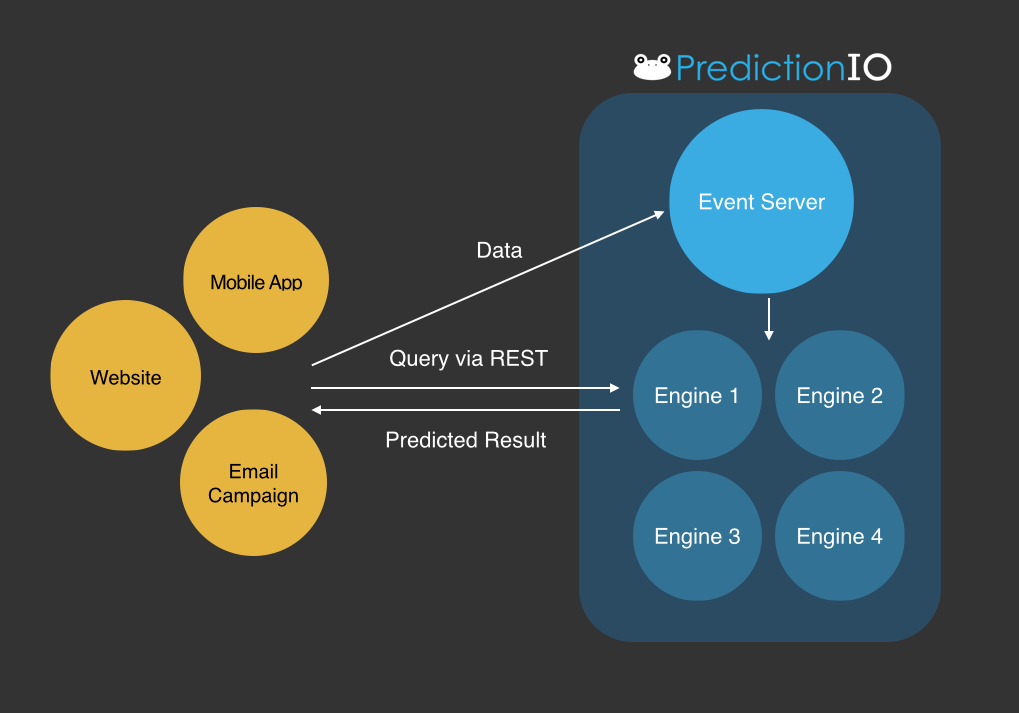
\includegraphics[scale=0.35]{images/predictionIO}
\caption{ How existing applications interact with PredictionIO \cite{predictionio}}
\label{fig:predictionIO}
\end{figure}


Figure \ref{fig:predictionIO} represents how PredictionIO is made to integrate with existing applications \cite{predictionio}. Data such as rating events from WOTM is sent to the Event Server where it is stored on PredictionIO. PredictionIO uses a distributed database that is easily scalable. Data from the event server is then used by algorithms from the engines to learn recommendations. These engines are deployed as distributed web services. WOTM can query these deployed engines to retrieve the top N recommendations for a specific user. 

The main advantage of using PredictionIO is that engines can be easily swapped out making it easy to examine and evaluate various CF techniques. This saves time, switching the main focus on CF algorithms rather than configuring settings to accommodate various technology and tools.

Additionally, these engines implement a DASE architecture. DASE stands for Data, Algorithms, Serving, and Evaluator. These components are considered to be independent in the engine which allows for separation of concerns. Implementation of various algorithms can be applied at the Algorithms stage, and enables results from the various algorithms to be combined at the Serving stage to produce hybrid CF approaches for recommendations.

PredictionIO already contains a range of customizable engines, including engines that use SVD techniques for CF. The PredictionIO community is active and new engines are frequently being produced. There is concise documentation in addition to support available. For these reasons, we found PredictionIO to be our best candidate and decided to use it. 

% \subsection{Online Learning vs Offline Learning}

% In a mobile application, speed and performance of recommendations is arguably more important than the prediction-accuracy. For instance, a user is more likely to use an application that provides fast recommendations to the users but less accurate recommendations, as opposed to an application that provides slow recommendations to the users but are accurate. In this case, the former is to be more accepted because users are able to easily skip inaccurate recommendations, whereas in the latter, users will have to wait for the recommendations to appear which may cause their attention to drift. 

% With this in consideration, it is important to provide fast recommendations to users, thus a model-based approaches would be more appropriate than neighbourhood methods. A model-based CF approach means that a model can be constructed and trained offline. Once the model is deployed, it will provide instant recommendations to the users because less computation needs to be done in real time, since the model has learnt what the user likes offline. As well as this, a model based approach means that expensive computation can be computed offline, providing high scalability. However, the disadvantage of a CF model based approach is that it must be regularly trained to take into account the recent new actions of the users. Therefore, regular intervals to train the model need to be defined depending on how often users rate dishes.

% Neighbourhood methods of CF perform online learning, meaning that they do the computation in real time. For instance, in user-based CF when a user likes a dish, then the algorithm will be performed then and there, finding similar users, then finding neighbours that are similar to that user, providing a recommendation. This technique is easy to implement, but does not scale well, and is slower than the modelled approach. However, depending on the size of data that is expected to be collected from this 'WOTM', it may be a valid approach if the data is not expected to be large (millions of ratings). As new users and new items grow in the application, it is expected that the amount of ratings will exponentially grow as well, therefore there is a possibility that scalability may have to be considered in the long term. As of now, we will focus on the performance of the recommender system.  

% For this reason, we will examine both online learning and offline learning, and see how implementations of the CF algorithm affect the performance of the recommendations that are produced.  


\subsection{User Experience}

A mobile application encourages user interaction that differs from that of a website. For instance, users are encouraged to use touch events to navigate through pages or to perform certain actions. This leads to design decisions that accommodate such interactions, making it easier for users to perform tasks on mobile applications. The user experience of WOTM affects how rating data is collected from users, which can affect the recommendation system. The following section explains the design decisions for collecting data events from users, and how these events can affect the recommender system. 

\subsection{Explicit Feedback}

Recommender systems rely on different types of input data \cite{koren2009matrix}. Explicit data is referred to as a direct record of someones interest of an item. For example, Netflix collects star ratings for movies, and TiVo users collect data from having a thumbs up or thumbs down directly indicating that they like or dislike a particular item \cite{koren2009matrix}. These events are mapped directly in the ratings matrix, and explain directly how a user feels about an item. 
The next section explains the design decisions regarding the explicit feedback we will collect in the WOTM application.

\subsubsection{Boolean Ratings vs Ternary Ratings vs Likert Scale Ratings}

Although prediction-accuracy is important, it is not the only factor that a recommender should focus on, and acts as one facet in wide range of facets \cite{martin2009recsys}. \citeauthor{martin2009recsys} explains that the goal of a recommender system is to improve user experience, however, designing a recommender system to fit a specific application remains a challenge, and recommender system ratings should be based on the user experience \cite{martin2009recsys}. By focusing on user experience, users will be able to easily rate food dishes, in turn, leading to the system collecting more information for the recommender system from ease of use. For this reason, a simple model allowing users to easily rate a dish such as a binary rating (Like/Neutral) or a ternary rating (like/neutral/dislike) is preferred over Likert scale ratings. This provides simplicity, but means recommendations will not be as accurate as Likert scale ratings such as 1-5 stars or 1-10 stars. By easing the user experience for rating food dishes it can increase data collection at the expense of accuracy. In fact, \citeauthor{movieratings} found that users provided more ratings that had options to ``like" or ``dislike" than users with only one rating option \cite{schafer2007collaborative, movieratings}. 

Using Likert scaled ratings mean that we learn more about the user preferences because of the scaled factor indicating how much the user likes a dish or not. This means that model based CF techniques are able to learn what the user likes and dislikes faster leading to more accurate recommendations. However, a Likert scale system such as a 1-5 star rating also has problems. For example, if a dish had a 5 star rating, it may mean only 1 or 2 people have rated the dish. Ratings such as 3.5 stars may mean that it is a good dish, but from the way it is displayed, may seem otherwise. \citeauthor{interface} explains that by displaying what other users think of an item, the active user tends be influenced by the opinions of others, leading to bias ratings \cite{interface}. An example would be a user rating a dish higher than they would normally because the food dish has an average of 4.5 stars. This can lead to inaccurate recommendations for the active user in the long term, because users may be influenced by others opinion \cite{interface}. \citeauthor{interface} argues that the way ratings are collected, and displayed influence how others will rate the dish. Considerations like this have to be taken into account to understand how the user will perceive and interact with the recommender system.  

A trade-off to consider is whether or not accurate recommendations are more important than the user experience. Since WOTM aims at being a mobile application, the limitations are the small form factor that mobile phone screens have. With a Likert scale rating system, the user has to be shown these possible options in order to rate a dish. This can take up additional space that is not available on small screens. Because of this, having a 1-5 star rating system may degrade the user experience as opposed to a simple like/dislike rating system. 

For a mobile application, the predicted score of the recommender system may not matter a great deal. For instance, a recommender system could predict two dishes the user may like based on previous rating patterns. The first dish is predicted with a 90\% predicted score, and the second dish is predicted with a 70\% predicted score that the user will like these dishes. But is the difference in prediction scores important if the user likes both dishes? As long as the recommender system has provided the user with dishes they like, the accuracy between those predicted dishes do not drastically matter. In addition, dishes with higher predicted scores may seem like obvious choices the user may have already tried, whereas dishes with a lower predicted score may lead to less obvious dishes that they may like, but have not tried yet. A recommender system using boolean or ternary values may eventually reach prediction accuracy similar to using likert scale ratings. Although this will happen in the long term, new ratings will most likely lead to less accurate predictions that join the system in the short term until more ratings are collected. 

Foursquare is an application that asks users to rate items according to a series of questions. These questions consist of ``What do you like about this place?", ``What is this place known for?" and so on. From these questions they are able infer a particular rating for the item, as well as collect data from users to give more accurate recommendations. This rating system may risk users not rating the items because of the long list of questions it asks. \cite{martin2009recsys} explains that part of the challenge is to design interfaces ``that give users control over the recommendation process without overwhelming the user or rendering the tool too complicated for novice users." 

For these reasons, we found that simple like/dislike events would best suit the collection of data for the recommender system because of the simplified structure which increases the user experience. The recommender system can be extended to take in additional events that may portray additional information such as a ``want" indicating that a user ``wants" a dish but has not yet tried it before. However, caution must be taken as more events will affect the user experience of the application, but may lead to more accurate recommendations. 

\subsection{Implicit Feedback}

When explicit feedback is not available, implicit data can be used to infer preferences from users \cite{koren2009matrix}. Implicit feedback is referred to as an indirect reflection of someones interest in an item. Implicit feedback can be from observing user behaviour. This could include click through data, browsing history, the way users react to certain events, search patterns, and so on \cite{koren2009matrix}. Implicit feedback can be collected to increase the accuracy of recommendations to users by being combined with explicit feedback, or can fill in the ratings matrix when explicit events are not available, alleviating the 'cold start' problem as it makes the matrix more dense. The next section explains design decisions regarding the implicit feedback in WOTM.

\subsubsection{Additional Events}

Netflix \cite{koren2009matrix} and other sites such as Amazon.com \cite{schafer2007collaborative} use implicit feedback such as views and purchase history in their recommender systems. These events indicate some form of interest in the user, however are less practical to apply for a mobile application. For example, on a website, many products are able to be shown to the user. When a user selects a product it will indicate some form of implicit feedback such as the user is interested in that product. With the WOTM mobile application, it can be difficult showing a range of food dishes to users because of the small screen size. This can make it difficult to collect additional implicit feedback. As well as this, purchase history and similar events are not practical because users are unlikely to indicate that they have purchased a dish after they have tried it. Explicit events such as like and dislike already infer that they have tried the dish, which make purchase history redundant. The implicit event of commenting on a dish may provide valuable information, perhaps commenting on a dish means that there is a strong interest or disinterest a user has about a specific dish. However, this is impractical because we do not know if the comment is good or bad without using extraction techniques.

A consideration is how to collect feedback on how the user feels about the recommendations produced by the recommender system. This can be used to gather more events, to make predictions more accurate. For instance, a user can indicate that they liked/disliked the recommendation that was shown to them, or they could skip it altogether meaning that they do not have an opinion about it. Although the flaw in this method is that recommendations may be dishes the user has not tried yet. Therefore, they may keep skipping through recommendations and provide no valid feedback to them. Although this may happen, an assumption is that user ``Like" events may be used for a dish that the user has not yet tried, but is interested in. 

For these reasons, we do not use any implicit events in our recommendation system.

\section{Implementation}

This section explains what has been implemented according to the design decisions in the previous section.


\subsection{Latent Factor Models}

PredictionIO \cite{predictionio} provides many template engines, some of which use CF algorithms to make recommendations to users. In particular, there is a template engine that uses Singular Value Decomposition, learning user preferences based on previous rating patterns. This engine is called the ``E-Commerce Recommendation Engine", and will be built upon to suit our user case. The following section explains the E-Commerce Recommendation Engine and the changes that have been made to it for this project. 

\subsubsection{E-Commerce Recommendation Engine}

The E-Commerce Recommendation Engine is written in the programming language Scala and is made to provide personalised recommendations for e-commerce applications. This engine uses Singular Value Decomposition which is a model-based CF technique. This means that the model trains on the users rating patterns to learn about recommendations that the users may be interested in. Training occurs offline. The engine also comes with the following out of the box functionality \cite{predictionio}.
\begin{enumerate}
 \item Exclude out-of-stock items
 \item Provide recommendation to new users who sign up after the model is trained
 \item Recommend unseen items only (configurable)
 \item Recommend popular items if no information about the user is available
\end{enumerate}

% TODO: REDO THIS
Default events in the engine are view events and purchase events.
Since ``view" and ``purchase" ratings are implicit events and not explicit events such as Likert scaled ratings from values 1-5, the implicit events have to be represented differently in the ratings matrix. An implicit event such as ``view" or ``purchase" event maps to a binary preference value of 1. Missing events map to a binary preference value of 0. 

A binary preference value of 1 indicates that the user likes the item, and a binary preference of 0 indicates no preference for the user. Additionally, implicit events also have a confidence value associated with it. These confidence values represent the confidence levels of the binary preference values being true. In this case, preference values for the ``view" and ``purchase" events correlate to the value of 1. Multiple identical events such as a user viewing the same item multiple times correlate to higher confidence levels since the confidence level is an aggregation of preference values. This means that there is a higher confidence level that the binary preference value is true, in this case, that the user will like the item because the user viewed or purchased the same item multiple times, recommendations taking this into account \todo{how? how can this be calculated?}. 

Singular Value Decomposition is then used with the same steps in equation \ref{eq:2}, except with a different minimization equation that considers the implicit events. This minimization equation is for implicit events which is the following \cite{implicit}.

\begin{equation}\label{eq:3}\tag{3}
\displaystyle min_{q*,p*} \sum_{ (u,i) \in K} c_{ui}(b_{ui} - q_{i}^T p_{u})^2 + \lambda (\| q_{i} \|^2 + \| p_{u} \|^2 )
\end{equation}

In this equation, \begin{math} c_{ui} \end{math} is the confidence level and \begin{math} b_{ui} \end{math} is the binary preference value. 

\subsubsection{Modifications to the Engine}

Using this template, we modified this engine to take into account ``Like" and ``Dislike" events, removing the view and purchase events. We modified the CF algorithm in the engine to consider a ``Like" event as positive result, giving it the preference value of a 1. In contrast, we made the algorithm in the engine consider a ``Dislike" event to be a negative result, giving it the preference value of a -1. Since users may be able change their minds about liking or disliking a dish, we modified the CF algorithm to only take into account the most recent like/dislike event that occurs from the user, if there are multiple identical like/dislike events on a dish from that user. Filtering in this recommendation system was also added. Users are now able to filter recommendations based on their preferences such as their meat type, their cuisine type, and their food type. As well as this, users can see recommendations that are within their price range, if specified. 

If dishes are no longer available, then we are able to send a query to the recommendation engine to tell it that the dish is unavailable. Another feature is that we are also able to send a query to the recommendation engine to say that a user has already seen that dish, and not to recommend that seen dish anymore. In this way, the user only sees new dishes that they have not been recommended yet.

This model recommends dishes to users as soon as they have liked a dish. These recommendations are also based on the ratings of other users rating patterns, which means that the ratings matrix should be dense. If the model cannot learn what the user likes, or the user has not rated anything yet, then it defaults to recommending the most popular dishes to the users. The advantage of this is that users get to see the trending dishes that other users prefer, however the disadvantage is that it may create bias results in the system because popular dishes will only be seen by new users. This means that new users will only rate the popular dishes, causing problems in the recommender engine. To extend this engine, we need to only recommend dishes to users after they have rated a certain number of dishes. Random dishes should be shown until they have rated a certain number of dishes. 

\todo{do yo use Cui?}

\section{Event Variations with SVD}

The use of different events can influence the recommendations that are provided by the system. For exmaple, using multiple explicit ratings such as Likes and Dislikes could affect the SVD algorithm. To understand how different events affect the recommender system, we implement variations of rating information is used with the SVD algorithm.

\subsection{SVD with Like events}

\subsection{SVD with Like and Dislike Events}

\subsection{Merging results from SVD with Like and Dislike events} 

Since SVD works by capturing latent factors of users and items using feature vectors, having the Like events and Dislike events in the same model, may correlate with each other but thus, be affected by the proportion of events since they are positive (likes) and negative (dislike) events. For example, if there is a larger amount of users that have disliked a specific item compared to the number of likes, the feature vector captured by that item may all correlate to negative values in the feature space. This may lead to inaccurate recommendations, where having another event such as ``Dislikes" actually deviates away from the main goal and can cause noisy information in the algorithm. For this reason, a more pratical approach in theory, would be to separate the different events in an independent SVD algorithm, and then combine the results from both algorithms at the end of the computation phase. We achieve this by defining a ``Like" and ``Dislike" with a value of 1.0. By defining positive values for ``Like" and ``Dislike" events, the idea is that the corresponding SVD algorithm will be able to recommend items that strongly correlate to the specfic event at the top. In this case, the algorithm corresponding to like events will display the top liked items for the active user, and the algorithm corresponding to the dislike events will display the top disliked items for the active users. We can then discount all the disliked recommendations from the list of liked recommendations, to provide higher accuracy with the users. 

\todo{explain implementation details?}



% \chapter{Future Plan}\label{C:future}


\section{Test methods}
\subsection{Evaluation Methods}



\section{Work Left}

\subsection{implement CF methods}


\section{Proposed Timeline}



\chapter{Evaluation}\label{C:evaluation}

\section{Experimental Objectives}
In this paper, we aim to compare a latent factor approach to collaborative filtering with a item-based collaborative filtering approach and a hybrid collaborative filtering approach. The main objectives are to answer the following questions:
\begin{itemize}
	\item{Do dislike events add value to the results to a latent factor model CF approach}
	\item{What are the best variations of using like and dislike events for a latent factor CF approach}
	\item{Do using user preferences add value to collaborative filtering}
	\item{Is item similarity CF more accurate than user based for latent factor models}
	\item{Is hybrid CF more accurate than user based for latent factor models}
	\item{Does filtering recommendations by a black list more accurate for latent factor models}
	\item{Does filtering based on preferences of the user, more accurate for latent factor models}
\end{itemize}

\subsection{Experimental Validity}

\subsection{Measurement Platform}

\section{Experimental Design}


\section{Methods?}

\subsection{User Dataset}

% \cite{martin2009recsys}
% Examples of this problem
% include the lack of standard treatment of items for which
% the recommender is unable to make a prediction. The broader
% goal of user-centered holistic evaluation, including A/B testing
% of the short- and long-term effects of recommendation differences,
% is still met by only a few research groups and companies
% that have the live systems and resources for such evaluation.

% Deploying innovative recommenders is still too hard, and there is a substantial need for research platforms where innovations can be tested without first building up a community of thousands of users. 
\todo{Show proportions of data}

\section{Experimental Setup}

\section{Issues}

\section{Offline Evaluation}

\subsection{Data Partitioning}

\subsection{Parameter Tuning}

\subsection{Offline Metrics}

\subsubsection{Binary List}

\subsubsection{Classification Accuracy}
\todo{do this}
Classification Accuracy Metrics. Classification metrics measure the
frequency with which a recommender system makes correct or incorrect decisions
about whether an item is good. Classification metrics are thus appropriate
for tasks such as Find Good Items when users have true binary preferences.
When applied to nonsynthesized data in offline experiments, classification
accuracy metrics may be challenged by data sparsity. The problem occurs when
the collaborative filtering system being evaluated is generating a list of top
recommended items. When the quality of the list is evaluated, recommendations
may be encountered that have not been rated. How those items are treated in
the evaluation can lead to certain biases.
One approach to evaluation using sparse data sets is to ignore recommendations
for items for which there are no ratings. The recommendation list is first
processed to remove all unrated items. The recommendation task has been altered
to “predict the top recommended items that have been rated.” In tasks
where the user only observes the top few recommendations, this could lead to
inaccurate evaluations of recommendation systems with respect to the user’s task. The problem is that the quality of the items that the user would actually
see may never be measured.

In essence, we are measuring how well the system
can identify items that the user was already aware of. This evaluation approach
may result in collaborative filtering algorithms that are biased towards obvious,
nonnovel recommendations or perhaps algorithms that are over fitted—fitting
the known data perfectly, but new data poorly.

Classification accuracy metrics do not attempt to directly measure the ability
of an algorithm to accurately predict ratings. Deviations from actual ratings
are tolerated, as long as they do not lead to classification errors. The particular
metrics that we discuss are Precision and Recall and related metrics and ROC.


\subsubsection{Precision \& Recall}
\todo {precision and recall}

Recall, in its purest sense, is almost always impractical to measure in a
recommender system. In the pure sense, measuring recall requires knowing
whether each item is relevant; for a movie recommender, this would involve
asking many users to view all 5000 movies to measure how successfully we recommend
each one to each user

Perhaps a more appropriate way to approximate precision and recall would
be to predict the top N items for which we have ratings. That is, we take a
user’s ratings, split them into a training set and a test set, train the algorithm
on the training set, then predict the top N items from that user’s test set. If we
assume that the distribution of relevant items and nonrelevant items within
the user’s test set is the same as the true distribution for the user across all
items, then the precision and recall will be much closer approximations of the
true precision and recall. This approach is taken in Basu et al. [1998].
In information retrieval, precision and recall can be linked to probabilities
that directly affect the user. If an algorithm has a measured precision of 70%,
then the user can expect that, on average, 7 out of every 10 documents returned
to the user will be relevant. Users can more intuitively comprehend the meaning
of a 10\% difference in precision than they can a 0.5-point difference in mean
absolute error

One of the primary challenges to using precision and recall to compare different
algorithms is that precision and recall must be considered together to
evaluate completely the performance of an algorithm.

Precision alone at a single search length or a single recall level can be appropriate
if the user does not need a complete list of all potentially relevant
items, such as in the Find Good Items task. If the task is to find all relevant
items in an area, then recall becomes important as well. However, the search
length at which precision is measured should be appropriate for the user task
and content domain.


\subsubsection{ROC Curves}

\subsubsection{Thresholding}

\section{Online Evaluation}

\section{Results}

\section{Limitations}

\section{Discussion}





\todo{Suggested Structure}

\section{Evaluation}

\subsection{Objectives}
\subsection{Threats to Validity}
\subsection{Design}
\subsubsection{Setup/Tools}
\subsubsection{Participants}
\subsubsection{Dataset}
\subsubsection{Method}
\subsection{Results}
\subsection{Limitations}
% %% $RCSfile: using.tex,v $
%% $Revision: 1.1 $
%% $Date: 2010/04/23 01:57:05 $
%% $Author: kevin $
%%
\chapter{Using this document and the \texttt{vuwproject} style}\label{C:us}

If you are writing an MSc or PhD thesis you should \emph{not} be using this style. Instead use \verb=vuwthesis=, which is based on the book style, and conforms to the VUW thesis rules. The thesis style is rather different from the project report style. 

This document is formatted using a local (to ECS and MSOR at VUW) style file. When you write your project report you should be very careful when changing the beginning. The document class settings should read:

\begin{verbatim}
\documentclass[11pt
              , a4paper
              , twoside
              , openright
              ]{report}
\end{verbatim}
The options to the document class specify that:
\begin{itemize}
\item 11pt font is to be used for the main body text,
\item  we will print on A4 paper, 
\item we will use duplex (two-sided) printing,
\item we want chapters to start on a right-hand page. 
\end{itemize}

The opitons you supply to the  \texttt{vuwproject} style will depend upon
what you are using the style for.

\subsection{Specifying the details}
The \texttt{vuwproject} style sets up the front page properly, and provides various commands allowing you to specify the author, title, supervisor or supervisors, the school from which the report is being submitted and the degree that the report is being submitted for. The style has deliberately been designed to do as little as possible. This means that your document can easily be re-formatted as a technical report, or for submission to a conference or journal by using the appropriate style.

It is also possible to use the style to easily produce documents on a
stand-alone computer where your \LaTeX installtion might not have all
of the  files and fonts available to machines within ECS or MSOR.

Most of the options to the \texttt{vuwproject} style are currently a simple
choice and there's a default that will make it obvious if you do not make
a choice.

Use one of the following options to use fonts available on ECS/MSOR machines
or to use images that imitate them (assumes you have copies of the images)
\begin{itemize}
\item \verb+font+
\item \verb+image+
\end{itemize}

Use one of the following options to set the school,
\begin{itemize}
\item \verb+ecs+
\item \verb+msor+
\end{itemize}

Use one of the following options to choose a pre-defined degree,
\begin{itemize}
\item \verb+bschonscomp+
\item \verb+mcompsci+
\end{itemize}

or use this command to use an explicit degree or diploma name
\begin{itemize}
\item \verb+\otherdegree{DEGREE OR DIPLOMA NAME}+
\end{itemize}

So, for example, to submit a report for the Master of Comp Sci degree, which
the style knows about, from within ECS, using the images, you'ld ensure the
 \texttt{vuwproject} line options looked like:

\begin{verbatim}
\usepackage[image,ecs,mcompsci]{vuwproject}
\end{verbatim}

whereas for a degree from within MSOR, when creating the final version on
an ECS or MSOR machine where you have access to the fonts, you would use
these options

\begin{verbatim}
\usepackage[font,msor]{vuwproject}
\end{verbatim}


and add the other degree's name using this command 

\begin{verbatim}
\otherdegree{DEGREE OR DIPLOMA NAME}
\end{verbatim}

To specify the supervisor or supervisors use either of the following commands in the preamble.
\begin{itemize}
\item \verb+\supervisor{The Supervisor}+
\item \verb+\supervisors{Super 1 and Super 2}+
\end{itemize}

If you fail to set any degree or supervisor, or the school, then the front page will report this.

The \texttt{vuwproject} style also sets the default font to be Palatino, using the \texttt{mathpazo} package. Palatino is one of VUW's `offical' fonts, and is the font used for the heading on the front page. The \texttt{mathpazo} package also typesets maths in a style which suits Palatino. 

\section{Copying the style}
If you want to write your project report away from VUW you will need to make your own copy of the \texttt{vuwproject} style.

You can find out where the original lives by reading the messages that \LaTeX\ prints when it is run.

Alternatively, you can down load a copy of the  \texttt{vuwproject} style from
the ECS webpages.

Any changes made to your own copy of the \texttt{vuwproject} style will not be reflected in the original, and \textit{vice versa}. Hence it makes sense to leave this as it is, and use a local style file for your own definitions.   

% \chapter{Some \LaTeX\ hints and tips}\label{C:ex}\LaTeX\ is a very good tool for producing well-structured documents carefully. It is very bad tool for banging things together in a rush and panic. \section{Floats}One perennial problem with \LaTeX\ is its treatment of \emph{floats}.  Suppose you have a figure or table which you want to include in your document. Where should it go? Traditional typesetting practice is to put these in some convenient place, such as the top or bottom of the current or next page, or at the end of the section or chapter.  \LaTeX\ adopts a similar strategy, and allows floats to ``float'' away from where they were defined. You can give a hint about where you want the figure, but \LaTeX\ may move it. Sometimes this is fine but sometimes you may want to have more control and insist that a float goes \emph{here}. Anselm Lingau's \textsf{float} package gives you this flexibility. For example, the following figure is an example of a non-floating float:\begin{fig}[H]
\begin{center}\begin{tabular}{l|lll}$\delta$ & $\mathit{a}$ & $\mathit{b}$ & $\Lambda$ \\ \hline $S_{1}$  & $\{\}$       & $\{\}$      & $\{S_{2}, S_{5}, S_{10}\}$\\$S_{2}$  & $\{S_{3}\}$  & $\{\}$      & $\{\}$\\$S_{3}$  & $\{S_{4}\}$  & $\{\}$      & $\{\}$\\$S_{4}$  & $\{S_{3}\}$  & $\{\}$      & $\{\}$\\$S_{5}$  & $\{\}$       & $\{S_{6}\}$ & $\{\}$\\$S_{6}$  & $\{\}$       & $\{S_{7}\}$ & $\{S_{8}\}$\\$S_{7}$  & $\{S_{6}\}$  & $\{\}$      & $\{\}$\\$S_{8}$  & $\{S_{9}\}$  & $\{\}$      & $\{\}$\\$S_{9}$  & $\{\}$       & $\{S_{8}\}$ & $\{\}$\\$S_{10}$ & $\{S_{11}\}$ & $\{\}$      & $\{\}$\\$S_{11}$ & $\{\}$       & $\{S_{10}\}$& $\{\}$\\ \end{tabular}\caption{The transition function of an NFA with $\Lambda$  transitions}

\end{center}
\end{fig}On the other hand, Figure \ref{Fig:two} is a floating float. 



\begin{fig}[tbh]
\begin{center}\begin{tabular}{l|ll}$\delta''$ & $\mathit{a}$ & $\mathit{b}$ \\ \hline $T_{1}$  & $T_{2}$ & $T_{3}$\\ $T_{2}$  & $T_{4}$ & $T_{5}$\\ $T_{3}$  & $T_{6}$ & $T_{7}$\\ $T_{4}$  & $T_{8}$ & \\$T_{5}$  & $T_{10}$ & \\$T_{6}$  &  & $T_{11}$\\ $T_{7}$  & $T_{3}$ & \\$T_{8}$  & $T_{4}$ & \\$T_{10}$  &  & $T_{5}$\\ $T_{11}$  & $T_{6}$ & \end{tabular}
\caption{The transition function of an FA to accept the same language.}\label{Fig:two}
\end{center}
\end{fig}You can define different types of new floats, and you can have tables of them in the contents pages.\section{URL's}Use \verb=\url= from the \textsf{url} package to typeset URL's. Just using \verb+\texttt+ or \verb+\tt+ does not work:\begin{itemize}\item \verb+\texttt{http://www.mcs.vuw.ac.nz/~neil/}+\item \verb+\url{http://www.mcs.vuw.ac.nz/~neil/}+\end{itemize}Give:\begin{itemize}\item \texttt{http://www.mcs.vuw.ac.nz/~neil/}\item \url{http://www.mcs.vuw.ac.nz/~neil/}\end{itemize}If you use the \textsf{hyperref} package then you can produce PDF files with clickable hyperlinks using \verb=\url=.\section{Graphics and \LaTeX}\LaTeX\ offers rather poor support for the inclusion of graphics. There are lots of ways to include pictorial material in \LaTeX, all of which are deficient in some way or other. Look at \cite{GRM97GC} for a description of them. If your document does need to have pictures in it it is worth thinking about what is needed \emph{before} you generate the pictures.\section{The bibliography}You should build up your bibliography as you go along.  Trying to get the details of the bibliography correct at the end of the project is hard work. Make sure that you record all the relevant details. Beware that material on the internet is likely to change very rapidly. If you are going to include material which is only available on the internet, then you should probably include in the reference the date on which you obtained the document.\section{Run \LaTeX, run}\LaTeX\ builds up information about your document for the table of contents, references and so on at each run. This means that, for example, the table of contents is really the table of contents of the previous compilation. You may need to run \LaTeX\ two or three times to let it catch up with itself. If you have cross references within your bibliography (for example two papers from the same collection, such as \cite{Dum93a,Dum93b}) you may need to run BibTeX more than once. It is also possible that the table of contents file has garbage in it, and will prevent the document from being compiled. This may happen if you have had to abort compilation, due to a bug in the source file. If this is the case then removing the \texttt{.toc} file will usually solve the problem. You will have to fix the original bug, of course.\section{Find out more by\ldots}You can find out more by:\begin{itemize}\item reading any one of a number of books, such as \cite{GMS94,Lam94}. The VUW library has copies of these;\item visiting  the Comprehensive \TeX\ Archive Network (CTAN) at \url{www.ctan.org};\item typing \texttt{latex} into Google.\end{itemize}It is \emph{highly unlikely} that you are the first person who ever wanted to do what you want to do with \LaTeX. Therefore it is likely that someone has already solved your problem: the real key to using  \LaTeX\ well is to make effective use of what other people have done.\section{Summary}In this chapter we explained some things about \LaTeX.
\chapter{Conclusions}\label{C:con}
The conclusions are presented in this Chapter.

\section{Contributions}
\begin{itemize}
	\item{Integrate CF with WOTM}
	\item{Develop three various CF}
	\item{Create dataset}
	\item{Evaluate and compare}
	\item{Percentage etc}
	\item{item popularity}
\end{itemize}

\section{Future Work}

\todo{IS USABLE HOW TO TEST (FUTURE WORK)?}

\subsection{User Evaluation or Online Evaluation}
In this experiment, we have identified the optimal parameters for each algorithm in order to do an online or user evaluation study. The next step is to conduct an online or user evaluation to see how users respond to the recommendations of each algorithm. From this, we are able to truly see how each algorithm performs in a real scenario, as well as test the novelty and serendipity factor and so forth. 

\subsection{Content-Based Filtering}
The content-based filtering approach we use with ALS is simple, yet effective. Currently each dish is categorised by three attributes and is manually labelled. In future work, depending on the attributes of the each food dish, we may want finer granularity, therefore, giving more precise content-based filtering recommendations based on preferences specified by users.  In future work, the content-based filtering approach may want to be treated as a classification problem, where machine learning algorithms will automatically label dishes based upon the contents of the dish and automatically learn what the user likes based on previous rating patterns. This can be used instead of the current approach where users explicitly label their preferences, which may interrupt the user experience of the application WOTM. In addition, pure content-based filtering approaches may want to be added into the hybrid collaborative filtering approach for the benefit of increasing the recommendation accuracy and relieving the ``Cold Start" problem CF suffers from. Although a hybrid CF approach can alleviate the cold start problem by using content-based filtering until there are enough ratings for accurate recommendations, the factors of complexity, scalability, and efficiency, must be considered when examining content-based filtering techniques. For example, algorithms such as Naive Bayes may be a good starting option since naive Bayes is efficient and generally gives good results, however, naive Bayes may need to run in real time to compute similar products when a user indicates they have liked a food dish, affecting the efficiency. These trade-offs have to be considered as each one may affect the user experience of the WOTM application. 

\subsection{Serendipity, Novelty, and Trust}
As mentioned earlier in Section \todo{do this}, serendipity and novelty are difficult to measure in offline evaluations. Trust is another factor difficult to measure in offline studies. In these cases, online evaluation or user studies may need to be conducted \todo{Check this}. Serendipity and Novelty are based on a form of randomness. This is used to help steer recommendations toward new items or serendipitous items. For example, in a KNN user based CF approach, serendipity or novelty may be adjusted depending on how many K neighbours (users) to take into account for. \todo{Considering a small number K neighbours, may lead to obvious recommendations for the current user, whereas choosing a higher number of K neighbours may lead to novel or serendipitous recommendations}. For future work, perhaps the ALS algorithm can be combined with a neighbourhood approach to provide some form of serendipity. Another approach that may help the hybrid approach in this paper, could be the adjustments of boost from the content-based filtering on the collaborative filtering approach. Higher boosted content values may lead to more obvious choices for the active user, whereas, lower approaches, would be similar in finding more serendipitous dishes based on other users ratings (CF).  

Trust also should be considered when factoring in novelty and serendipity into the recommendation engine. New users to the application of WOTM, may test the recommendation system to establish trust before they start using the application regularly. In future work, this should be taken into account, and should also be tested in online studies. For example, a recommendation engine that tries to provide new users with novel or serendipitous food dishes may invoke less trust and confidence for the new users. This may eventually lead to new users not trusting the system, and abandoning the application, or disregarding any of the personalised recommendations given. In order to combat this, future work should provide the most obvious choices to the users (perhaps by boosting the content), and then as time progresses, start introducing novel and serendipitous recommendations to the users. In addition, the application may allow users to set the settings for these users, enabling user specific goals to be accomplished. 

\subsection{Contextual events}
In future work, context events provide more information to the recommendation engine in terms of the device the user is using to access the application, and the location of where the active user is. Another way that may make the recommendation more accurate is to use user search content. This would require adding a search engine which would then index all the users searches to provide a boost of recommendations based on the content or food dish searched for. This context information should boost the strength of the collaborative filtering search, and also have a decaying factor since the context of the events have purpose behind it. For example, on a hot day, a user may want ice cream and search for it. But on the next day, they may want feel like something new. For these reasons, a decaying factor should be added into the engine.

\section{Conclusion}
\begin{appendices}

\chapter{Results from Evaluation} \label{appendix:results_table}
Contents of each run from the evaluation section where the second method is applied. 

\begin{figure}
\centering
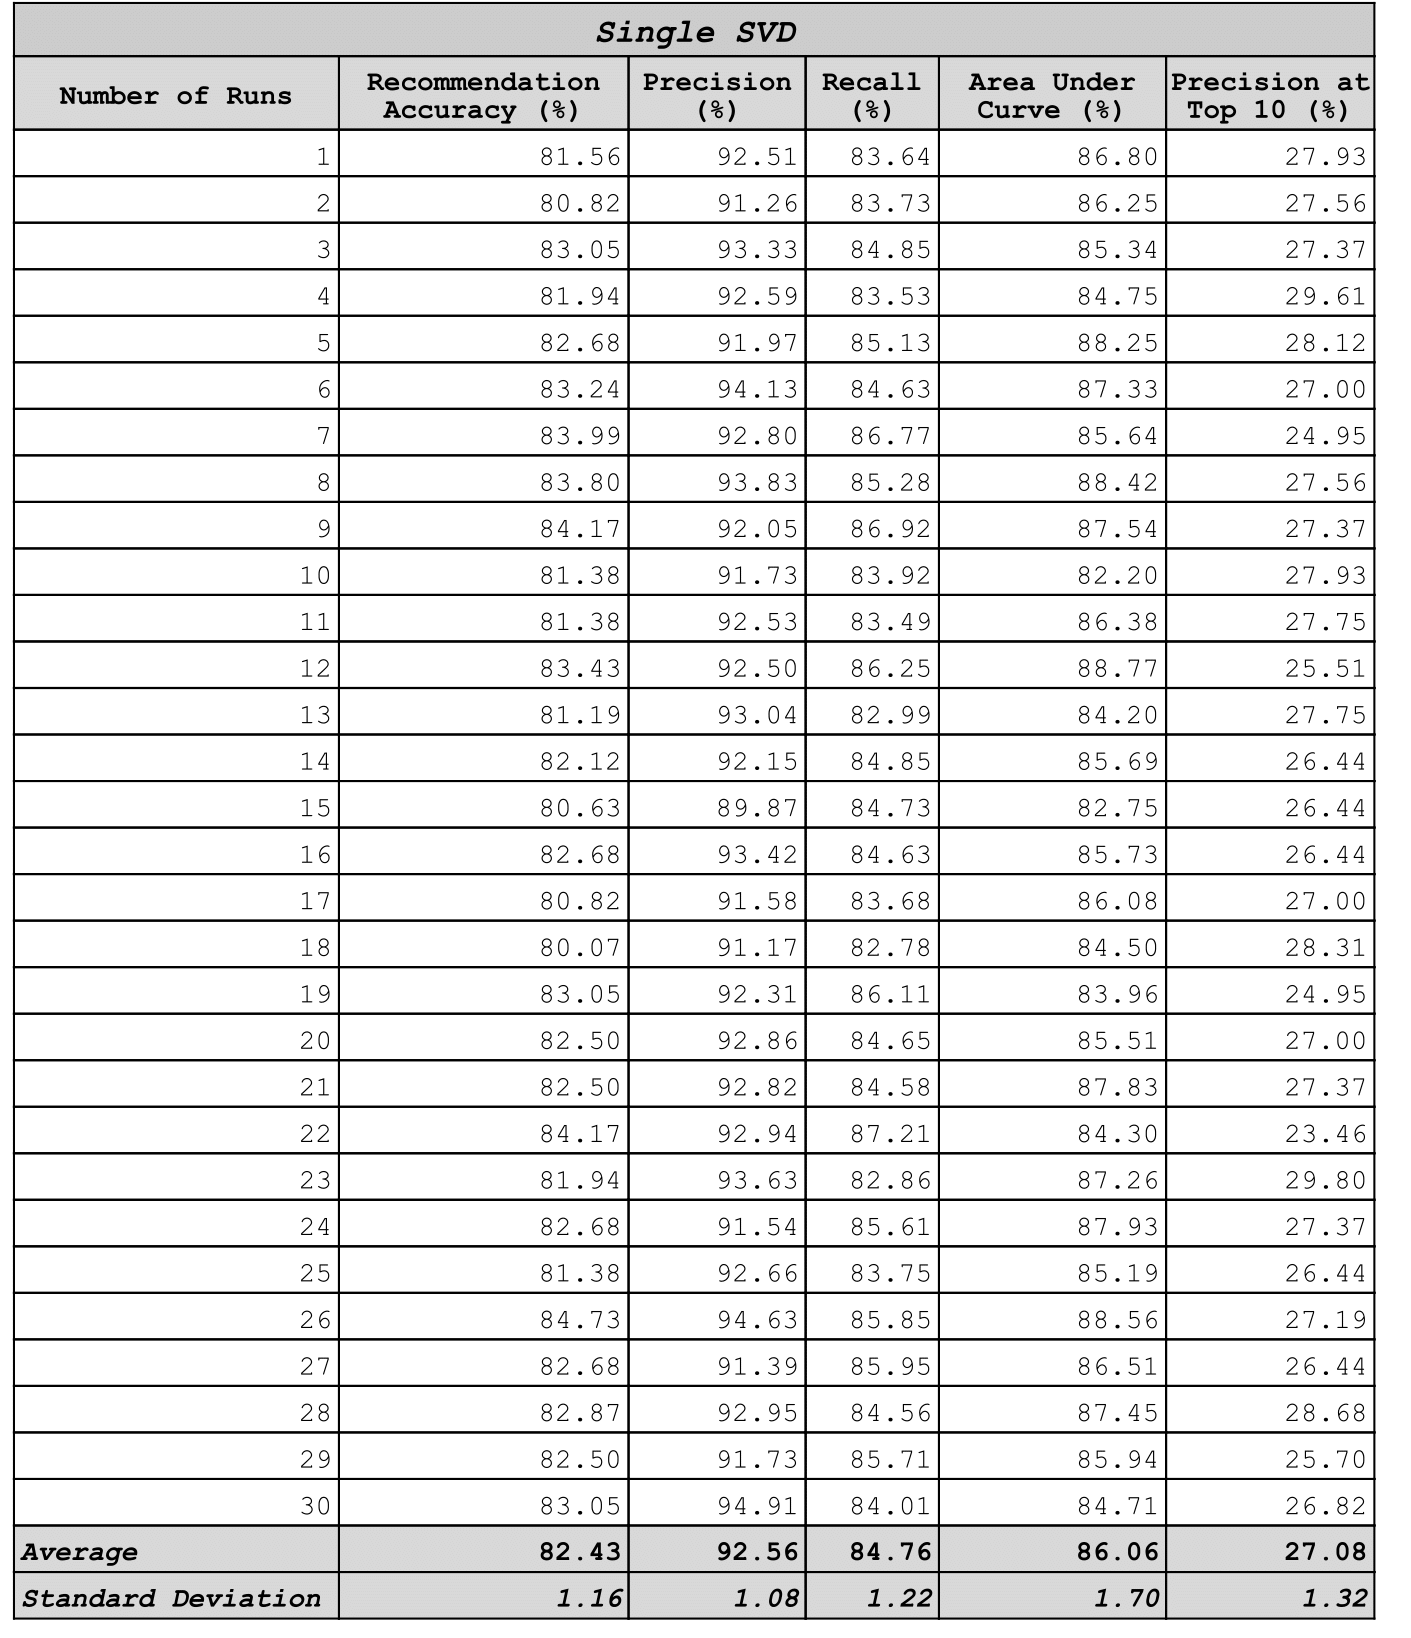
\includegraphics[scale=0.3]{appendices/single_als_30_runs.png}
\caption{Individual 30 runs of the Single SVD system.}
\label{fig:single_algorithm}
\end{figure}

\begin{figure}
\centering
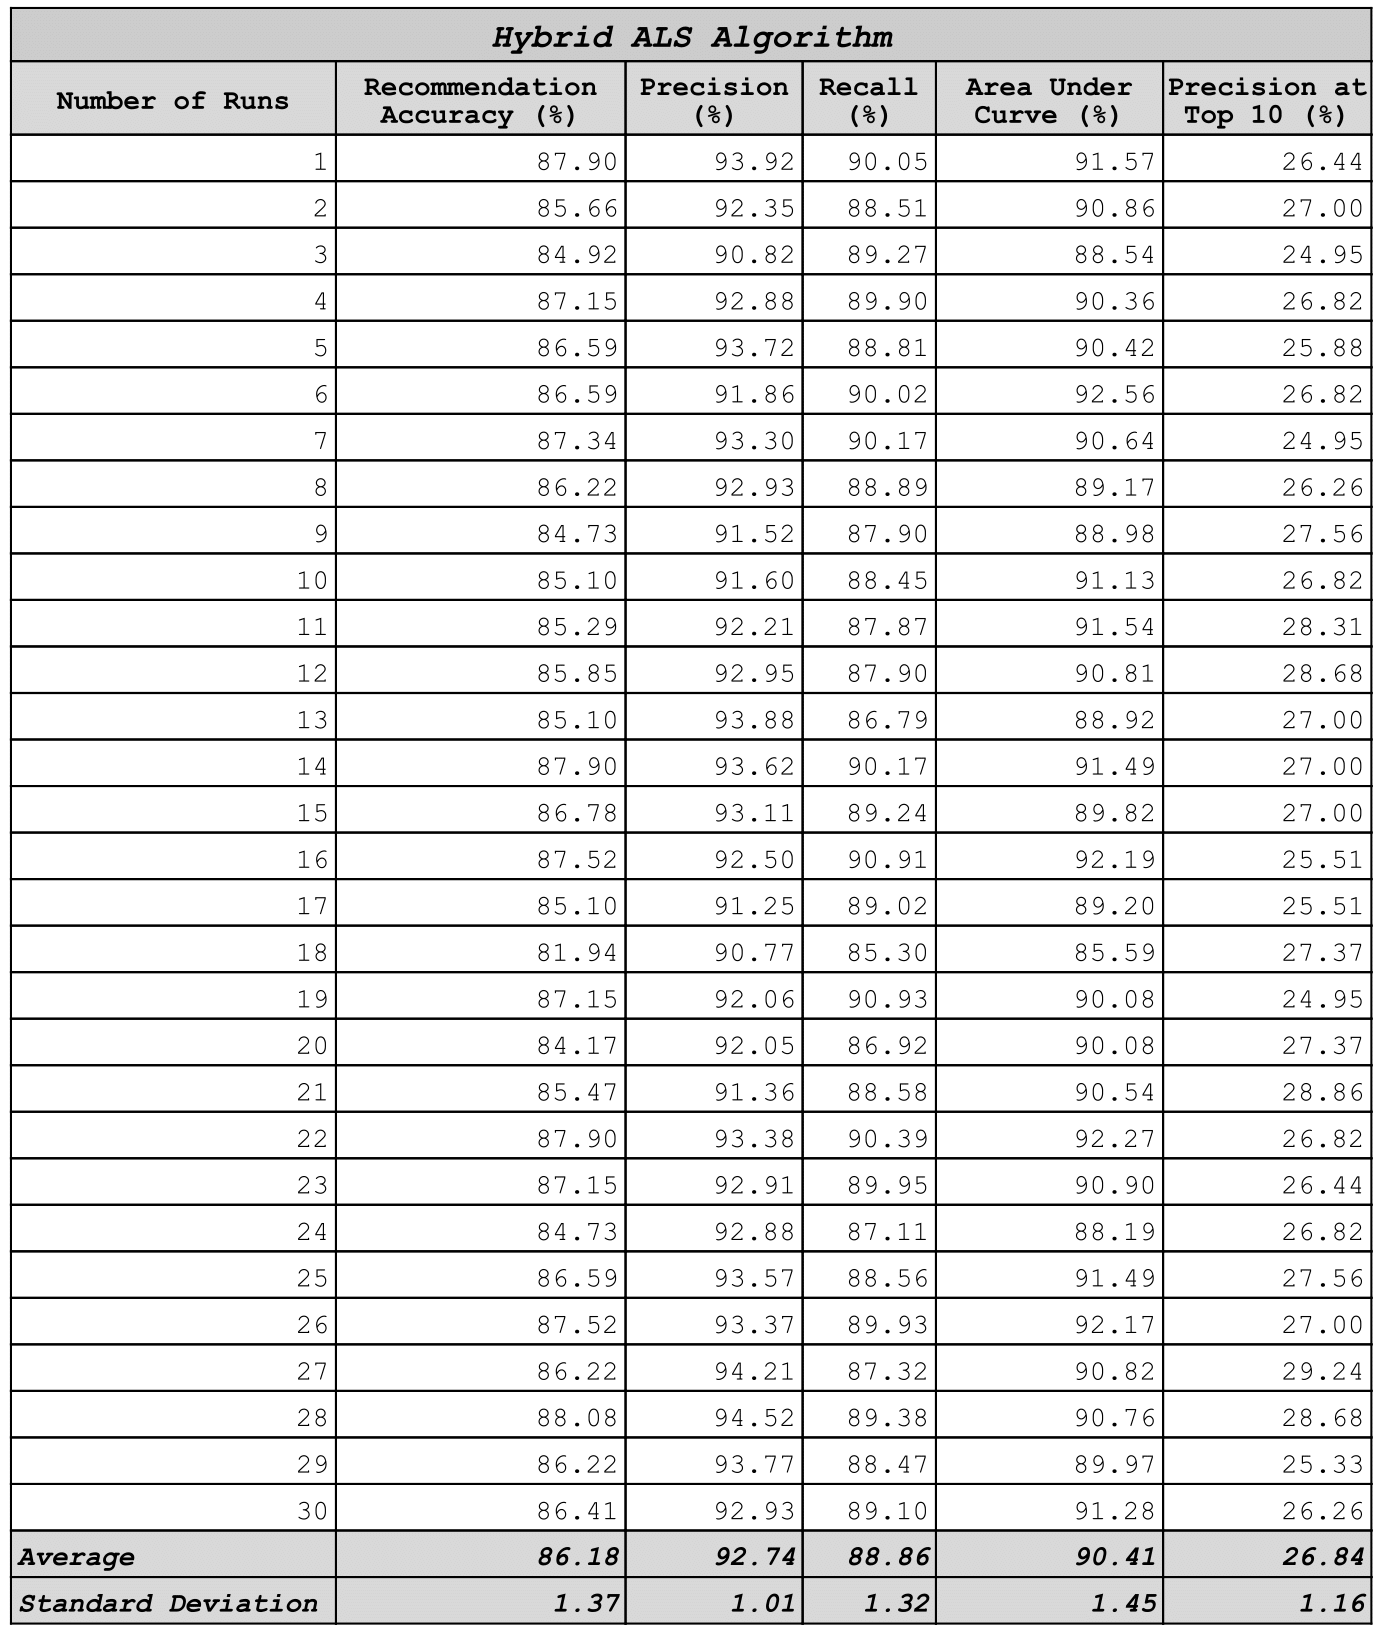
\includegraphics[scale=0.3]{appendices/hybrid_als_30_runs.png}
\caption{Individual 30 runs of the Hybrid SVD algorithm which takes into account the content preferences of the user and considers these preferences when making recommendations.}
\label{fig:dual_algorithm}
\end{figure}

\begin{figure}
\centering
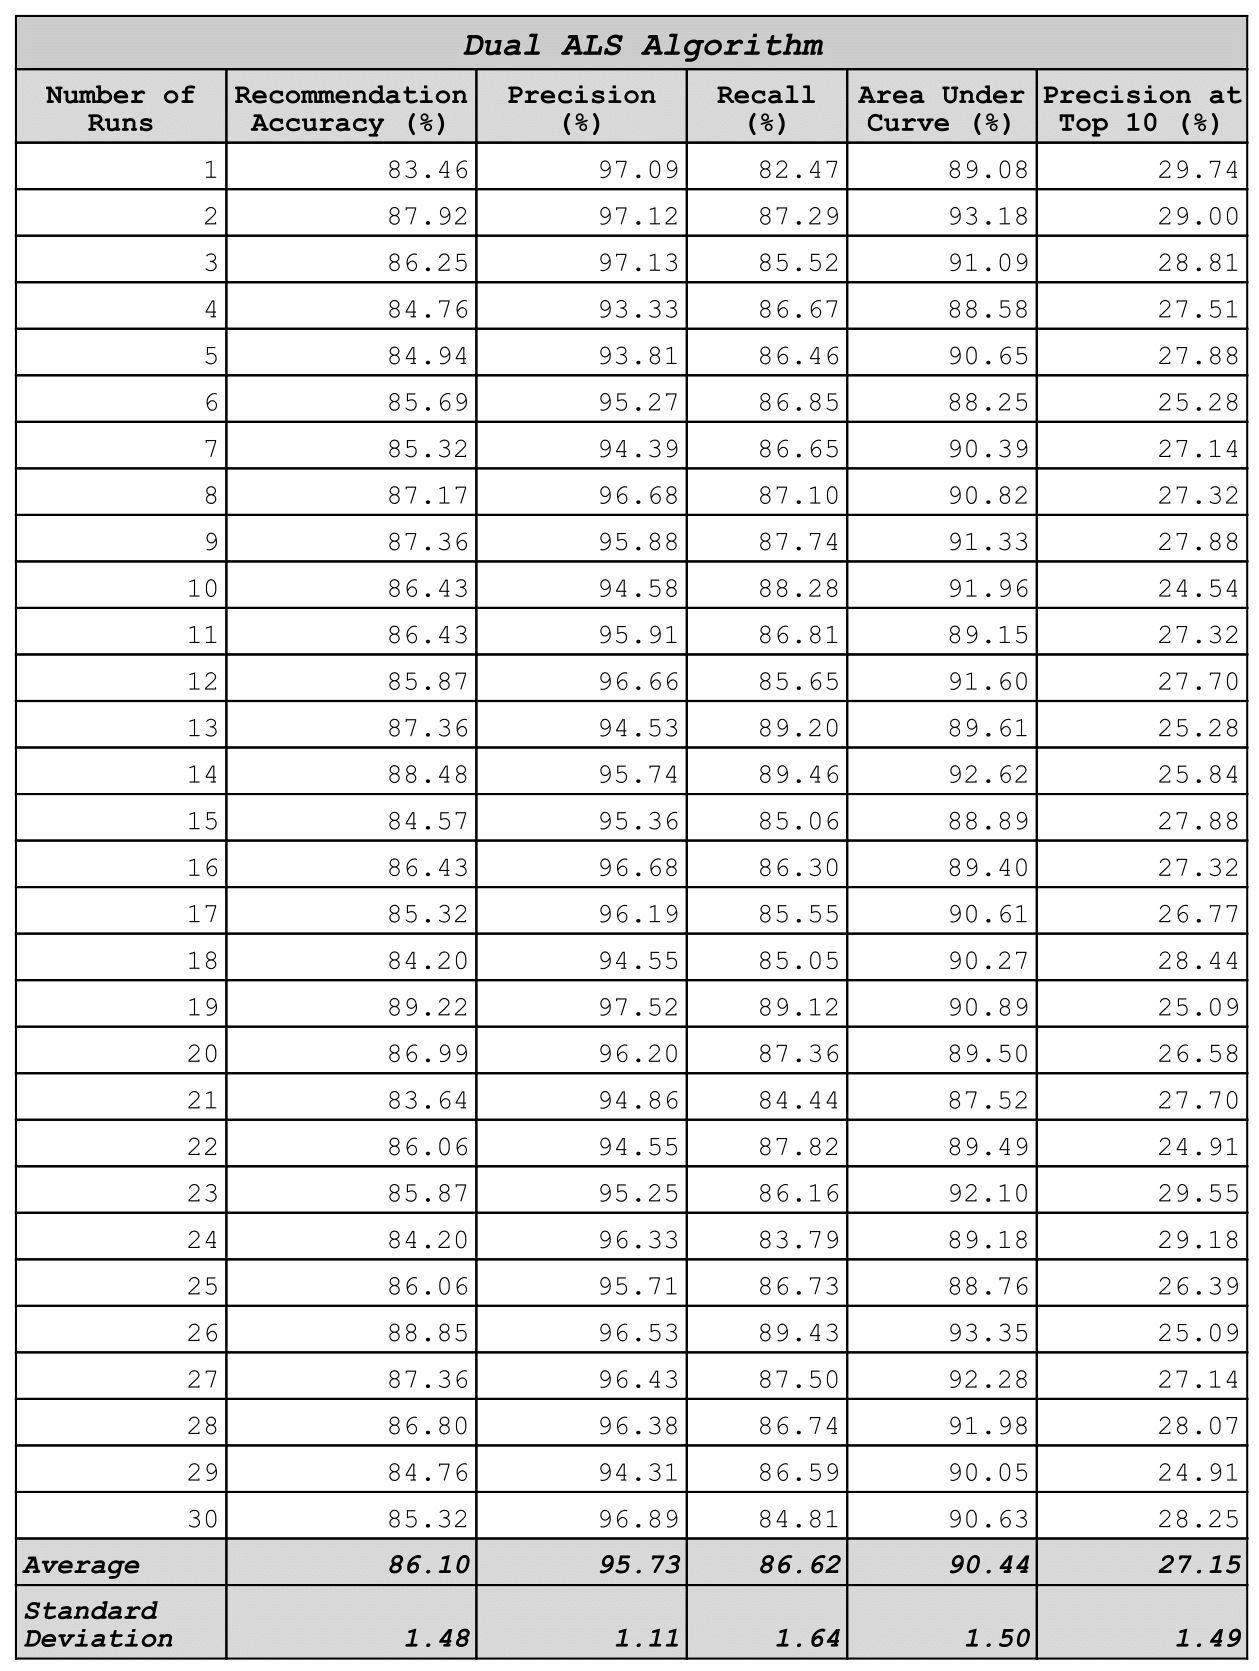
\includegraphics[scale=0.3]{appendices/dual_als_30_runs.png}
\caption{Individual 30 runs of the dual SVD system. }
\label{fig:dual_algorithm}
\end{figure}

\begin{figure}
\centering
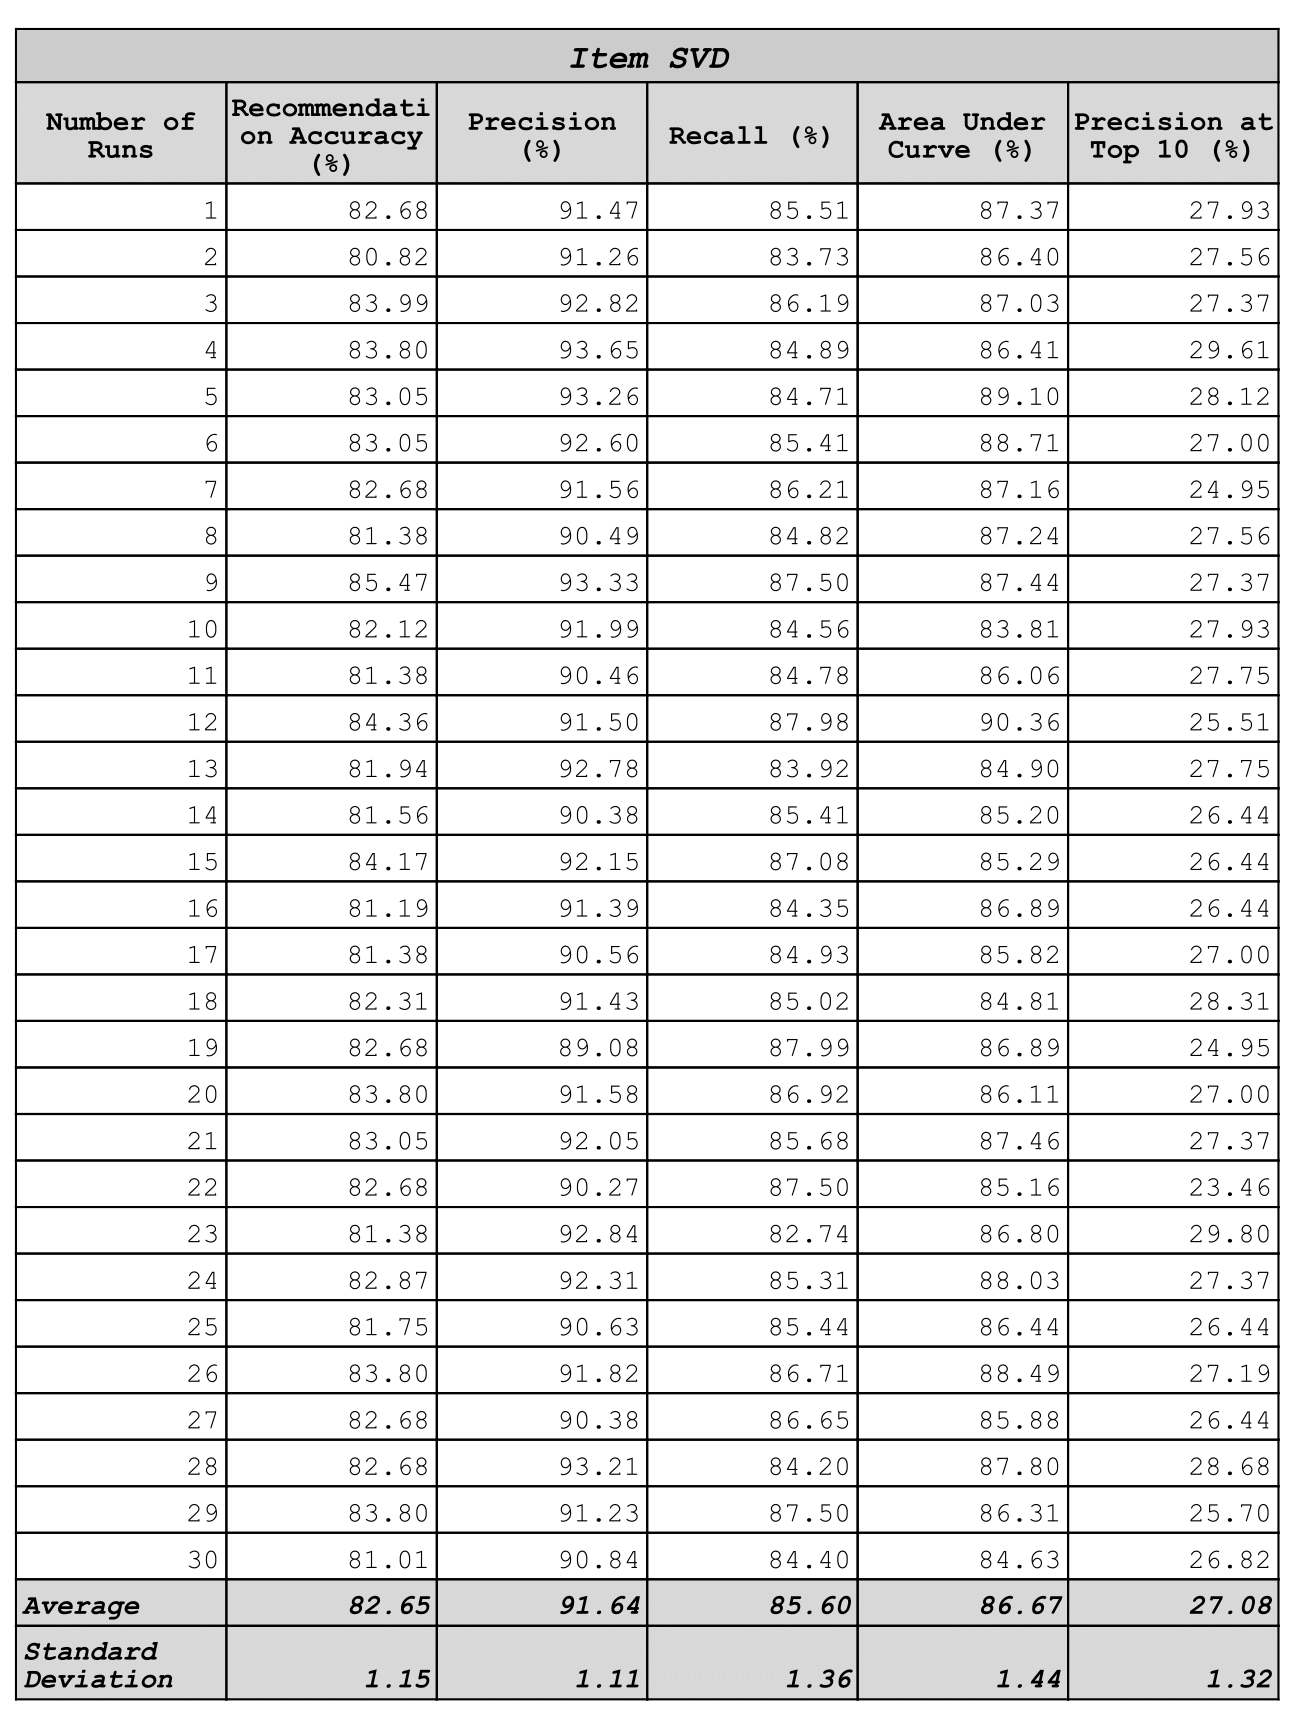
\includegraphics[scale=0.3]{appendices/item_als_30_runs.png}
\caption{Individual 30 runs of the Item SVD system. }
\label{fig:dual_algorithm}
\end{figure}

\begin{figure}
\centering
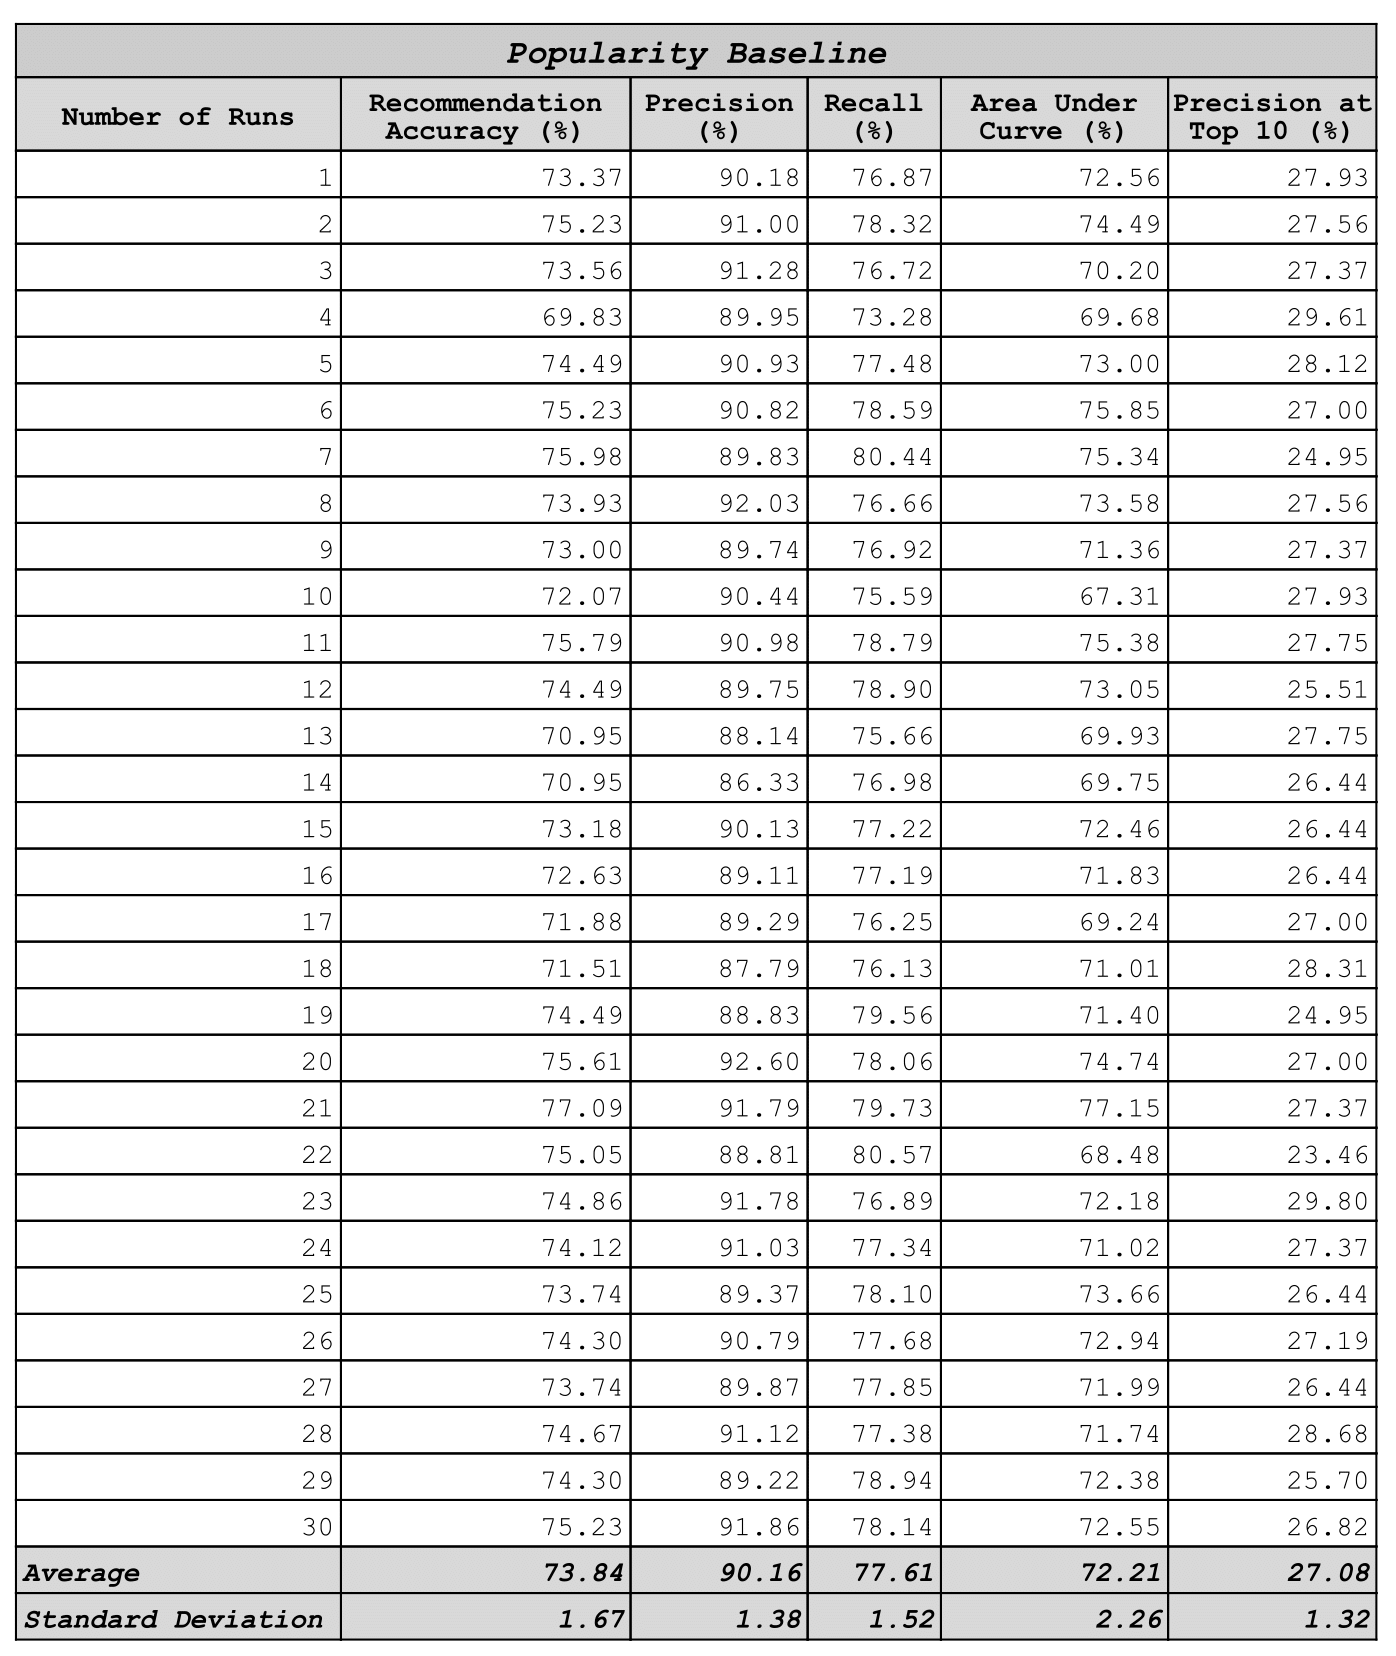
\includegraphics[scale=0.3]{appendices/popular_30_runs.png}
\caption{Individual 30 runs of Baseline Predictor based on item popularity (non-personalised recommendations). }
\label{fig:dual_algorithm}
\end{figure}

\chapter{Survey} \label{appendix:survey}

Contents of the user study. 

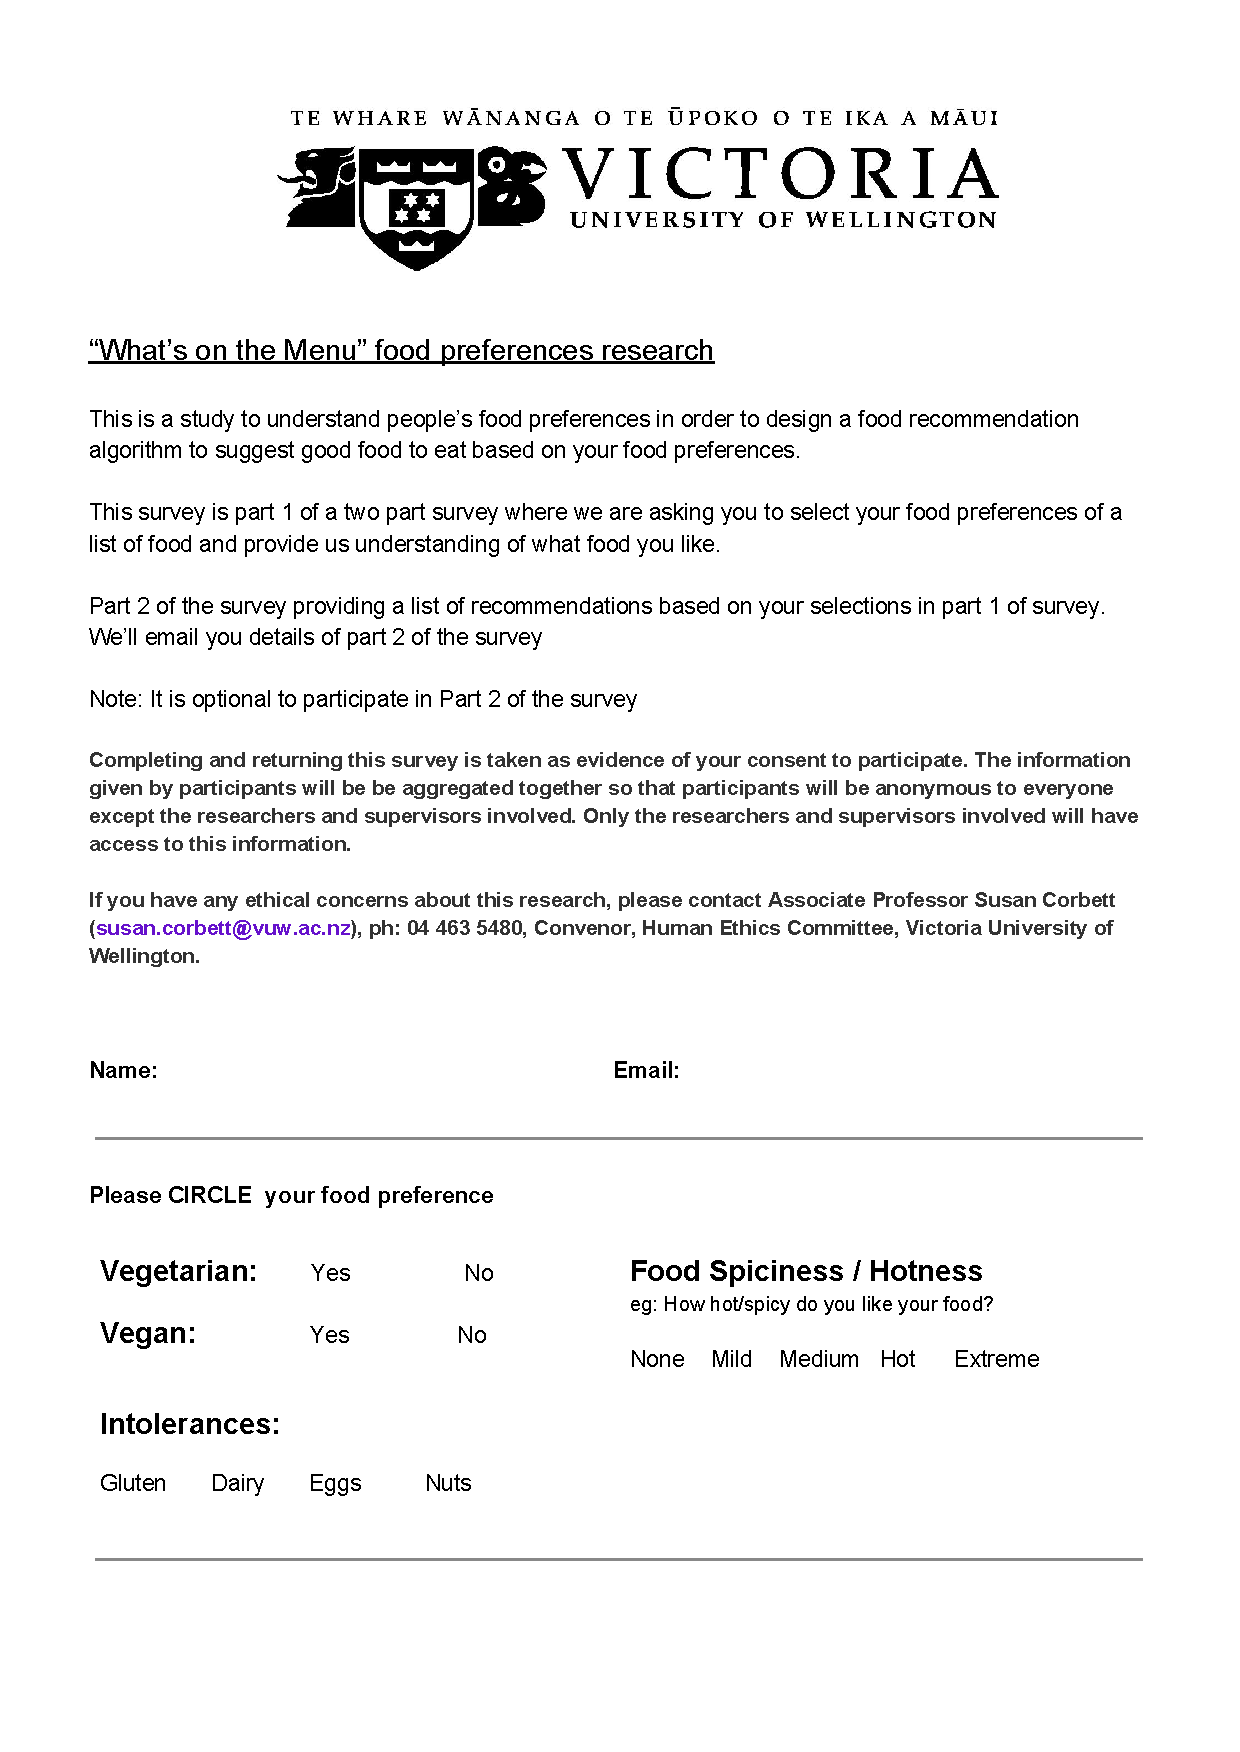
\includepdf[pages={1-2}]{appendices/survey_1.pdf}
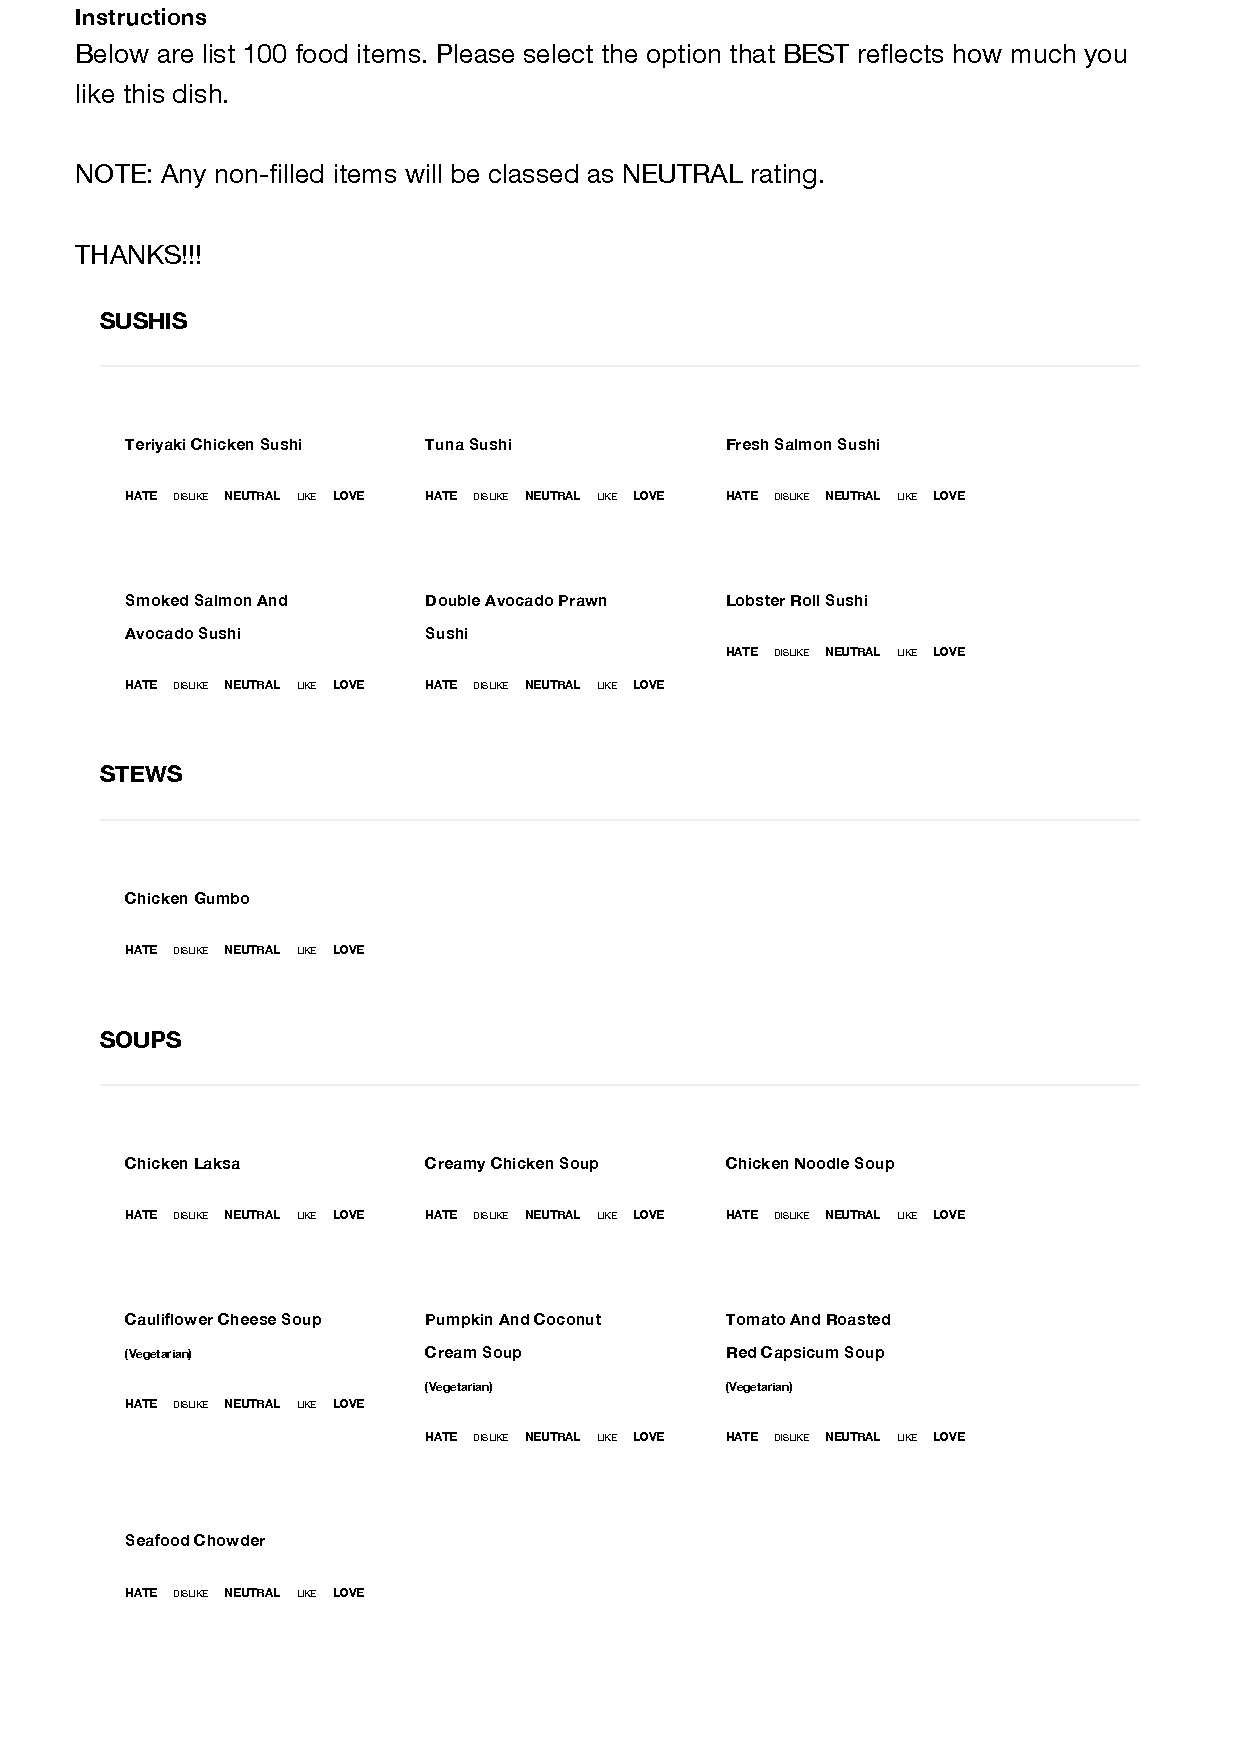
\includepdf[pages={1-7}]{appendices/survey_2.pdf}

\chapter{Human Ethics Committee (HEC)} \label{appendix:hec}

Contents of the Human Ethics Committee, including approval.

\begin{figure} 
\centering
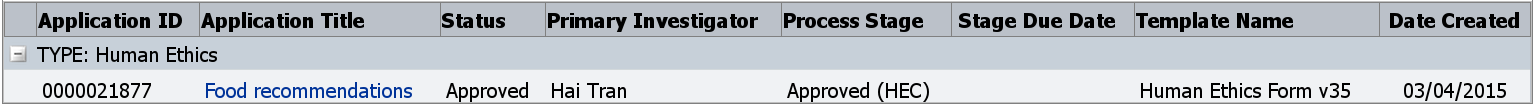
\includegraphics[scale=0.3]{appendices/hec_approval.png}
\caption{Human Ethics Approval for the experiment.}
\label{fig:hec_approval}
\end{figure}


\includepdf[pages={1-2}]{appendices/participant_form.pdf}

\end{appendices}



%%%%%%%%%%%%%%%%%%%%%%%%%%%%%%%%%%%%%%%%%%%%%%%%%%%%%%%

\backmatter

%%%%%%%%%%%%%%%%%%%%%%%%%%%%%%%%%%%%%%%%%%%%%%%%%%%%%%%


% % \bibliographystyle{ieeetr}
% \bibliographystyle{acm}

\bibliography{sample}
\bibliographystyle{IEEEtranN/IEEEtranN}

% \nocite{*}

\end{document}
